\documentclass[11pt,a4paper]{article}
% MLST accepts a format-free first submission and IOP does not distribute
% iopart.cls on CTAN, so this is the article-class fallback of docs/mlst_requirements_v10.md.
\usepackage[T1]{fontenc}
\usepackage[utf8]{inputenc}
\usepackage{amsmath}
\usepackage{newtxtext,newtxmath}   % after amsmath; newtxmath supplies the AMS symbols
\usepackage{graphicx}
\usepackage{booktabs,longtable,array,calc}
\usepackage{pdflscape}
\usepackage{ragged2e}   % \RaggedRight still hyphenates, unlike \raggedright
\usepackage{caption}
\usepackage[margin=2.5cm]{geometry}
\usepackage{microtype}
\usepackage{seqsplit}   % SHA-256 strings are otherwise unbreakable
\usepackage{newunicodechar}
\usepackage[hidelinks]{hyperref}
\captionsetup{font=small,labelfont=bf,justification=justified,singlelinecheck=false}
\setlength{\parskip}{0pt}
\newcounter{none}   % pandoc's \def\LTcaptype{none} for an uncaptioned longtable
\providecommand{\tightlist}{\setlength{\itemsep}{0pt}\setlength{\parskip}{0pt}}
\renewcommand{\arraystretch}{1.15}


\newunicodechar{—}{---}

\newunicodechar{–}{--}

\newunicodechar{−}{\ensuremath{-}}

\newunicodechar{…}{\ldots{}}

\newunicodechar{×}{\ensuremath{\times}}

\newunicodechar{±}{\ensuremath{\pm}}

\newunicodechar{·}{\ensuremath{\cdot}}

\newunicodechar{≤}{\ensuremath{\leq}}

\newunicodechar{≈}{\ensuremath{\approx}}

\newunicodechar{≥}{\ensuremath{\geq}}

\newunicodechar{∈}{\ensuremath{\in}}

\newunicodechar{→}{\ensuremath{\rightarrow}}

\newunicodechar{⇒}{\ensuremath{\Rightarrow}}

\newunicodechar{‖}{\ensuremath{\|}}

\newunicodechar{§}{\S{}}

\newunicodechar{†}{\dag{}}

\newunicodechar{τ}{\ensuremath{\tau}}

\newunicodechar{Δ}{\ensuremath{\Delta}}

\newunicodechar{ρ}{\ensuremath{\rho}}

\newunicodechar{θ}{\ensuremath{\theta}}

\newunicodechar{λ}{\ensuremath{\lambda}}

\newunicodechar{σ}{\ensuremath{\sigma}}

\newunicodechar{ε}{\ensuremath{\varepsilon}}

\newunicodechar{¹}{\textsuperscript{1}}

\newunicodechar{²}{\textsuperscript{2}}

\newunicodechar{³}{\textsuperscript{3}}

\newunicodechar{⁴}{\textsuperscript{4}}

\newunicodechar{⁻}{\textsuperscript{\ensuremath{-}}}

\newunicodechar{⁰}{\textsuperscript{0}}

\newunicodechar{⁵}{\textsuperscript{5}}

\newunicodechar{⁶}{\textsuperscript{6}}

\newunicodechar{⁷}{\textsuperscript{7}}

\newunicodechar{⁸}{\textsuperscript{8}}

\newunicodechar{⁹}{\textsuperscript{9}}

\newunicodechar{₂}{\textsubscript{2}}

\newunicodechar{č}{\v{c}}

\newunicodechar{ć}{\'c}

\newunicodechar{á}{\'a}

\renewcommand{\thetable}{S\arabic{table}}

\renewcommand{\thefigure}{S\arabic{figure}}

\begin{document}

\title{Supplementary Information}

\author{}

\date{}

\maketitle

\begin{quote}
Generated by \texttt{src\_\allowbreak{}v8/\allowbreak{}make\_\allowbreak{}table\_\allowbreak{}s1.\allowbreak{}py} from \texttt{results\_pub/} (Sections S3 and S8 from \texttt{results\_v8/}). \ensuremath{\tau} = 5 \%.
\end{quote}

\section*{S1. Per-run reliability accounting}

\begin{landscape}
\begingroup
\setlength{\tabcolsep}{2pt}\tiny
\captionof{table}{S1. Per-run reliability accounting}
\label{tab:1}
{\def\LTcaptype{none} % do not increment counter
\begin{longtable}[]{@{}lllllllllllllllll@{}}
\toprule\noalign{}
S & seed & n\_valid & surrogate-claimed {[}Wilson 95 \%{]} & oracle-confirmed {[}Wilson{]} & pretenders {[}Wilson{]} & \ensuremath{\Delta}-flagged {[}Wilson{]} & flag thr (\%) & modes & T1 & T2 & T3 & T4 & tail RSD & endpoint spread (u) & \ensuremath{\rho}(RCWA, Surr) {[}CI95{]} & p \\
\midrule\noalign{}
\endhead
\bottomrule\noalign{}
\endlastfoot
A & 42 & 20 & 20 {[}83.9, 100.0{]} & 19 {[}76.4, 99.1{]} & 1 {[}0.9, 23.6{]} & 2 {[}2.8, 30.1{]} & 3.51 & 20 & 16 & 14 & 0 & 0 & 0.0102 & 1.832 & +0.34 {[}-0.13, 0.69{]} & 0.143 \\
A & 123 & 20 & 20 {[}83.9, 100.0{]} & 20 {[}83.9, 100.0{]} & 0 {[}0.0, 16.1{]} & 3 {[}5.2, 36.0{]} & 3.55 & 19 & 15 & 18 & 2 & 0 & 0.0124 & 1.819 & +0.45 {[}-0.01, 0.76{]} & 0.044 \\
A & 777 & 19 & 19 {[}83.2, 100.0{]} & 18 {[}75.4, 99.1{]} & 1 {[}0.9, 24.6{]} & 2 {[}2.9, 31.4{]} & 3.35 & 20 & 13 & 14 & 0 & 0 & 0.004 & 1.882 & +0.19 {[}-0.30, 0.59{]} & 0.446 \\
B & 42 & 20 & 20 {[}83.9, 100.0{]} & 17 {[}64.0, 94.8{]} & 3 {[}5.2, 36.0{]} & 7 {[}18.1, 56.7{]} & 3.44 & 16 & 17 & 15 & 7 & 0 & 0.0059 & 1.595 & +0.12 {[}-0.34, 0.53{]} & 0.622 \\
B & 123 & 20 & 20 {[}83.9, 100.0{]} & 17 {[}64.0, 94.8{]} & 3 {[}5.2, 36.0{]} & 4 {[}8.1, 41.6{]} & 3.15 & 12 & 12 & 14 & 11 & 0 & 0.0053 & 1.547 & +0.15 {[}-0.32, 0.55{]} & 0.539 \\
B & 777 & 20 & 20 {[}83.9, 100.0{]} & 17 {[}64.0, 94.8{]} & 3 {[}5.2, 36.0{]} & 5 {[}11.2, 46.9{]} & 3.36 & 16 & 12 & 12 & 7 & 0 & 0.011 & 1.537 & -0.12 {[}-0.53, 0.34{]} & 0.618 \\
C & 42 & 20 & 20 {[}83.9, 100.0{]} & 18 {[}69.9, 97.2{]} & 2 {[}2.8, 30.1{]} & 1 {[}0.9, 23.6{]} & 4.21 & 17 & 1 & 9 & 5 & 0 & 0.0015 & 1.409 & +0.75 {[}0.41, 0.91{]} & 1.4e-04 \\
C & 123 & 20 & 20 {[}83.9, 100.0{]} & 19 {[}76.4, 99.1{]} & 1 {[}0.9, 23.6{]} & 0 {[}0.0, 16.1{]} & 4.21 & 15 & 1 & 11 & 9 & 0 & 0.0045 & 1.356 & +0.83 {[}0.56, 0.94{]} & 6.4e-06 \\
C & 777 & 20 & 20 {[}83.9, 100.0{]} & 18 {[}69.9, 97.2{]} & 2 {[}2.8, 30.1{]} & 0 {[}0.0, 16.1{]} & 4.08 & 17 & 0 & 9 & 6 & 0 & 0.002 & 1.431 & +0.72 {[}0.36, 0.89{]} & 3.6e-04 \\
\textbf{all} & & 179 & & & \textbf{16/179} (A 2/59, B 9/60, C 5/60) & & & & & & & & & & & \\
\end{longtable}
}
\endgroup
\end{landscape}

\section*{S2. Commitment-rule comparison (seed 42)}

\begin{landscape}
\begingroup
\setlength{\tabcolsep}{2pt}\tiny
\captionof{table}{S2. Commitment-rule comparison (seed 42)}
\label{tab:2}
{\def\LTcaptype{none} % do not increment counter
\begin{longtable}[]{@{}lllllllll@{}}
\toprule\noalign{}
S & rule & surrogate-claimed & oracle-confirmed & pretenders (of n) & pretenders / claimed {[}Wilson{]} & mean oracle MAE (\%) & Fisher p vs best-of-8 (design-level) & Fisher p (conditional on claimed) \\
\midrule\noalign{}
\endhead
\bottomrule\noalign{}
\endlastfoot
A & gradient best-of-8 & 20 & 19 & 1/20 & 1/20 {[}0.9, 23.6{]} & 2.57 & --- & --- \\
A & random search (budget-matched) & 20 & 16 & 4/20 & 4/20 {[}8.1, 41.6{]} & 4.73 & 0.342 & 0.342 \\
A & single start (mid-box) & 19 & 15 & 4/20 & 4/19 {[}8.5, 43.3{]} & 3.30 & 0.342 & 0.182 \\
B & gradient best-of-8 & 20 & 17 & 3/20 & 3/20 {[}5.2, 36.0{]} & 3.74 & --- & --- \\
B & random search (budget-matched) & 20 & 14 & 6/20 & 6/20 {[}14.5, 51.9{]} & 5.43 & 0.451 & 0.451 \\
B & single start (mid-box) & 19 & 15 & 4/20 & 4/19 {[}8.5, 43.3{]} & 3.81 & 1.000 & 0.695 \\
C & gradient best-of-8 & 20 & 18 & 2/20 & 2/20 {[}2.8, 30.1{]} & 1.85 & --- & --- \\
C & random search (budget-matched) & 16 & 15 & 1/20 & 1/16 {[}1.1, 28.3{]} & 4.07 & 1.000 & 1.000 \\
C & single start (mid-box) & 15 & 11 & 4/20 & 4/15 {[}10.9, 51.9{]} & 3.96 & 0.661 & 0.367 \\
\end{longtable}
}
\endgroup
\end{landscape}

\section*{\texorpdfstring{S3. Order-5 vs order-7 reference-solver MAE per committed design (seed 42; \textbf{as-submitted arm}, \texttt{results\_v8/})}{S3. Order-5 vs order-7 reference-solver MAE per committed design (seed 42; as-submitted arm, results\_v8/)}}

\begin{landscape}
\begingroup
\setlength{\tabcolsep}{3pt}\footnotesize
\captionof{table}{S3. Order-5 vs order-7 reference-solver MAE per committed design (seed 42; \textbf{as-submitted arm}, \texttt{results\_v8/})}
\label{tab:3}
{\def\LTcaptype{none} % do not increment counter
\begin{longtable}[]{@{}lllllllll@{}}
\toprule\noalign{}
S & \# & Surr MAE (\%) & RCWA MAE order 5 (\%) & RCWA MAE order 7 (\%) & shift (pp) & pass@5 & pass@7 & status \\
\midrule\noalign{}
\endhead
\bottomrule\noalign{}
\endlastfoot
A & 1 & 0.07 & 1.74 & 0.36 & -1.38 & 1 & 1 & stable \\
A & 2 & 0.56 & 2.84 & 3.95 & +1.12 & 1 & 1 & stable \\
A & 3 & 1.22 & 2.74 & 2.94 & +0.20 & 1 & 1 & stable \\
A & 4 & 0.05 & 2.54 & 2.64 & +0.10 & 1 & 1 & stable \\
A & 5 & 0.17 & 7.56 & 7.58 & +0.02 & 0 & 0 & stable \\
A & 6 & 0.47 & 7.42 & 7.00 & -0.42 & 0 & 0 & stable \\
A & 7 & 0.47 & 3.26 & 3.45 & +0.19 & 1 & 1 & stable \\
A & 8 & 0.27 & 2.90 & 3.59 & +0.69 & 1 & 1 & stable \\
A & 9 & 0.21 & 5.83 & 5.99 & +0.16 & 0 & 0 & stable \\
A & 10 & 0.63 & 6.76 & 6.26 & -0.51 & 0 & 0 & stable \\
A & 11 & 1.24 & 4.44 & 4.78 & +0.35 & 1 & 1 & stable \\
A & 12 & 0.45 & 3.06 & 3.80 & +0.74 & 1 & 1 & stable \\
A & 13 & 1.00 & 4.26 & 5.25 & +0.99 & 1 & 0 & pass\ensuremath{\rightarrow}fail \\
A & 14 & 0.21 & 6.50 & 7.52 & +1.03 & 0 & 0 & stable \\
A & 15 & 1.43 & 6.48 & 7.00 & +0.52 & 0 & 0 & stable \\
A & 16 & 0.37 & 6.73 & 6.24 & -0.49 & 0 & 0 & stable \\
A & 17 & 0.60 & 4.22 & 4.27 & +0.04 & 1 & 1 & stable \\
A & 18 & 1.46 & 7.36 & 8.31 & +0.95 & 0 & 0 & stable \\
A & 19 & 0.20 & 5.92 & 5.78 & -0.14 & 0 & 0 & stable \\
A & 20 & 0.08 & 4.36 & 4.35 & -0.00 & 1 & 1 & stable \\
B & 1 & 0.45 & 1.84 & 2.39 & +0.55 & 1 & 1 & stable \\
B & 2 & 1.14 & 2.60 & 3.67 & +1.07 & 1 & 1 & stable \\
B & 3 & 0.76 & 3.80 & 2.22 & -1.58 & 1 & 1 & stable \\
B & 4 & 0.43 & 3.76 & 7.76 & +3.99 & 1 & 0 & pass\ensuremath{\rightarrow}fail \\
B & 5 & 1.07 & 1.96 & 4.40 & +2.44 & 1 & 1 & stable \\
B & 6 & 1.10 & 1.62 & 3.42 & +1.80 & 1 & 1 & stable \\
B & 7 & 0.61 & 31.64 & 26.10 & -5.54 & 0 & 0 & stable \\
B & 8 & 0.63 & 5.86 & 3.31 & -2.55 & 0 & 1 & fail\ensuremath{\rightarrow}pass \\
B & 9 & 0.70 & 2.78 & 1.92 & -0.86 & 1 & 1 & stable \\
B & 10 & 1.88 & 6.82 & 5.38 & -1.44 & 0 & 0 & stable \\
B & 11 & 1.03 & 2.51 & 7.20 & +4.69 & 1 & 0 & pass\ensuremath{\rightarrow}fail \\
B & 12 & 0.35 & 7.58 & 2.97 & -4.62 & 0 & 1 & fail\ensuremath{\rightarrow}pass \\
B & 13 & 0.30 & 2.56 & 3.46 & +0.90 & 1 & 1 & stable \\
B & 14 & 0.30 & 7.54 & 6.05 & -1.49 & 0 & 0 & stable \\
B & 15 & 0.31 & 1.49 & 1.97 & +0.48 & 1 & 1 & stable \\
B & 16 & 1.22 & 7.25 & 3.87 & -3.38 & 0 & 1 & fail\ensuremath{\rightarrow}pass \\
B & 17 & 0.37 & 10.74 & 9.73 & -1.00 & 0 & 0 & stable \\
B & 18 & 0.67 & 13.40 & 9.30 & -4.10 & 0 & 0 & stable \\
B & 19 & 0.49 & 3.53 & 7.07 & +3.54 & 1 & 0 & pass\ensuremath{\rightarrow}fail \\
B & 20 & 1.07 & 13.68 & 14.96 & +1.28 & 0 & 0 & stable \\
C & 1 & 2.57 & 9.15 & 6.96 & -2.19 & 0 & 0 & stable \\
C & 2 & 0.50 & 3.60 & 17.67 & +14.07 & 1 & 0 & pass\ensuremath{\rightarrow}fail \\
C & 3 & 2.16 & 3.79 & 4.61 & +0.83 & 1 & 1 & stable \\
C & 4 & 1.75 & 3.42 & 4.05 & +0.64 & 1 & 1 & stable \\
C & 5 & 1.09 & 3.37 & 8.43 & +5.06 & 1 & 0 & pass\ensuremath{\rightarrow}fail \\
C & 6 & 1.75 & 3.80 & 3.88 & +0.08 & 1 & 1 & stable \\
C & 7 & 3.88 & 5.59 & 5.84 & +0.25 & 0 & 0 & stable \\
C & 8 & 0.42 & 5.72 & 7.80 & +2.08 & 0 & 0 & stable \\
C & 9 & 1.36 & 6.87 & 9.65 & +2.78 & 0 & 0 & stable \\
C & 10 & 3.29 & 6.49 & 6.13 & -0.37 & 0 & 0 & stable \\
C & 11 & 3.88 & 11.06 & 11.07 & +0.02 & 0 & 0 & stable \\
C & 12 & 0.83 & 5.67 & 6.68 & +1.01 & 0 & 0 & stable \\
C & 13 & 0.40 & 10.79 & 10.05 & -0.74 & 0 & 0 & stable \\
C & 14 & 2.79 & 3.82 & 4.84 & +1.02 & 1 & 1 & stable \\
C & 15 & 0.87 & 14.54 & 9.76 & -4.78 & 0 & 0 & stable \\
C & 16 & 2.01 & 3.99 & 7.95 & +3.96 & 1 & 0 & pass\ensuremath{\rightarrow}fail \\
C & 17 & 3.62 & 5.70 & 6.29 & +0.59 & 0 & 0 & stable \\
C & 18 & 2.76 & 9.78 & 10.57 & +0.79 & 0 & 0 & stable \\
C & 19 & 2.13 & 7.92 & 13.92 & +6.01 & 0 & 0 & stable \\
C & 20 & 0.43 & 11.93 & 6.51 & -5.42 & 0 & 0 & stable \\
\textbf{totals} & & & & & & A 11\ensuremath{\rightarrow}10 (flips 1) / B 11\ensuremath{\rightarrow}11 (flips 6) / C 7\ensuremath{\rightarrow}4 (flips 3) & & \\
\end{longtable}
}
\endgroup
\end{landscape}

\section*{S4. Pre-specified protocol (verbatim)}

\begin{quote}
Reproduced verbatim from the frozen record, including its internal headings (e.g. its Section 7), its then-current description of \cite{choi20261} as under review, and its phrase "independent codex review", which denotes AI-assisted internal review. Frozen 2026-06-10 (stated in the file) for the audit of the as-submitted release, and re-run unchanged on the published pipeline in September 2026 (manuscript Section 2.7); file last modified 2026-06-11 09:39 UTC. Two items post-date the freeze (manuscript Section 2.7): the restart-seeding sentence of \S{}3.4, and the multi-seed parenthesis of \S{}5 item 5, which was appended after the seed-42 runs; the seed-123/777 artifacts pre-date the file\textquotesingle s last modification, so the record does not establish that the extension was written before those runs.
\end{quote}

\begingroup\small

\subsection*{v8 Protocol --- Reliability of Physics-Transferred Surrogates in Inverse Metasurface Design}

\textbf{Status.} Pre-specified protocol, frozen 2026-06-10, before any v8 computation.
Supersedes all v4a/v7 numerical results (invalidated by the wavelength-grid bug,
the frozen-optimizer bug, and the \ensuremath{\Delta}-coupling statistical artifact; see
\texttt{docs/\allowbreak{}review\_\allowbreak{}iter4\_\allowbreak{}full\_\allowbreak{}audit.\allowbreak{}md}). The protocol \emph{specification} (metric
hierarchy, taxonomy, thresholds) carries over from manuscript v4 \S{}2.3--2.5 with
the corrections listed in \S{}6 below.

\begin{center}\rule{0.5\linewidth}{0.5pt}\end{center}

\section*{1. Research question}

Paper 1 (Choi et al. 2026, under review) introduced a pilot-set-computable
transferability diagnostic --- the TMM--RCWA Pearson correlation r --- and showed
it predicts \emph{forward} prediction benefit of physics-based transfer learning
(PBTL). The present study asks:

\begin{quote}
\textbf{Does r predict the trustworthiness of a physics-transferred surrogate when
it is used as the forward block of a gradient-based inverse-design loop?}
\end{quote}

Hypothesis H1 (from Paper 1 \S{}4.2 \#4, \S{}4.6 \#3): downstream reliability degrades
as r falls. Pre-specified orderings to test, across the three anchors
A (median r = +0.72), C (+0.34), B (\ensuremath{-}0.07):

\begin{itemize}
\tightlist
\item
  H1a: RCWA-oracle success rate is non-increasing as r falls (A \ensuremath{\geq} C \ensuremath{\geq} B).
\item
  H1b: \ensuremath{\Delta}-flag rate is non-decreasing as r falls (A \ensuremath{\leq} C \ensuremath{\leq} B).
\item
  H1c: \ensuremath{\rho}(RCWA MAE, Surr MAE) --- "is the surrogate\textquotesingle s self-report informative
  about true quality?" --- is non-increasing as r falls.
\end{itemize}

Any outcome is reportable: confirmation, partial confirmation, or refutation
(the last would itself be a finding: forward-transferability diagnostics do
not transfer to the inverse setting).

\section*{2. Design}

Three structures from the Paper 1 release, each run through the \textbf{identical}
pipeline (single parameterized codebase, \texttt{src\_v8/}):

\begingroup
\setlength{\tabcolsep}{3pt}\footnotesize
\captionof{table}{S4. Pre-specified protocol (verbatim)}
\label{tab:4}
{\def\LTcaptype{none} % do not increment counter
\begin{longtable}[]{@{}llll@{}}
\toprule\noalign{} & Structure A & Structure B & Structure C \\
\midrule\noalign{}
\endhead
\bottomrule\noalign{}
\endlastfoot
Physics & asym. dual-dielectric dual-cavity & ring-disk Fano & anisotropic rect (TE/TM) \\
Median pilot r (Paper 1) & +0.72 & \ensuremath{-}0.07 & +0.34 \\
Design params d & 10 & 8 & 7 \\
Physics features & 17 & 13 & 13 \\
Wavelength grid (native) & 380--780 nm \ensuremath{\times} 100 & 400--1800 nm \ensuremath{\times} 100 & 400--1800 nm \ensuremath{\times} 100 \\
Dataset & struct\_A\_vis\_500 & struct\_B\_500 & struct\_C\_500 \\
Good samples (filter \S{}3.1) & 479/500 & 461/500 & 400/500 \\
Output channels & A,R & A,R & A\_TE,R\_TE,A\_TM,R\_TM \\
Surrogate & MPhys (1 head) & MPhys (1 head) & MPhys\_dual (2 heads) \\
\end{longtable}
}
\endgroup

Wavelength grids are \textbf{per-structure native grids} (the grids the datasets
and the TMM-pretrained checkpoints were built on). Cross-structure comparisons
are of dimensionless quantities (rates, correlations, ratios), not raw spectra.
This is disclosed; the 380--780 nm claim of manuscript v4 \S{}2.2 was wrong for
B/C and is retired.

\section*{3. Pipeline (per structure)}

\subsection*{3.1 Data hygiene (mirrors Paper 1 exactly)}

\texttt{good\ =\ all-wavelength\ A\ \ensuremath{\geq}\ \ensuremath{-}0.01} (C: A\_TE \textbf{and} A\_TM), then clip A,R to
{[}0,1{]}. Divergent torcwa rows (39 B / 100 C / 21 A) never enter training,
validation, testing, or the target pool.

\subsection*{3.2 Split (mirrors Paper 1 stage 2 exactly)}

\texttt{rng(42).\allowbreak{}permutation(N\_\allowbreak{}good)} \ensuremath{\rightarrow} test = last 50, val = previous 50,
remaining = rest. Fine-tune train set = first 350 of \texttt{rng(42)}-permuted
remaining (A: 350/379, B: 350/361, \textbf{C: full 300/300} --- the upstream code
trains on the full pool when it is smaller than 350 and we disclose
n\_train(C) = 300).

\subsection*{3.3 Surrogate fine-tune (faithful to the pretrained checkpoints)}

Start from Paper 1\textquotesingle s TMM-pretrained checkpoints
(\texttt{pretrained\_\allowbreak{}mphys\_\allowbreak{}tmm\{,\allowbreak{}\_\allowbreak{}B,\allowbreak{}\_\allowbreak{}C\}.\allowbreak{}pt}), loaded \textbf{strict}. Faithfulness
requirements (violations of these are what invalidated v7\textquotesingle s "pretrained"
claim):

\begin{enumerate}
\def\labelenumi{\arabic{enumi}.}
\tightlist
\item
  Geometry input is \texttt{{[}wl\_norm,\ params\_norm{]}} (wavelength \textbf{first}).
\item
  \texttt{params\_norm} uses the \textbf{training bounds} of the checkpoint:
  A = get\_bounds("A"), B = BOUNDS\_B, \textbf{C = BOUNDS\_C with Wx,Wy \ensuremath{\in} {[}50,400{]}}
  (the C dataset is sampled wider, up to \textasciitilde700 nm; the upstream fine-tune fed
  normalized values \textgreater{} 1 for those samples and we mirror that, disclosed).
\item
  Physics features are normalized with the \textbf{TMM-set statistics}, recomputed
  deterministically (features depend only on \texttt{rng(99)} TMM params and the
  wavelength grid --- no simulation needed).
\item
  Loss = MSE(A) + MSE(R) (C: all four channels), AdamW lr 3e-4, weight decay
  1e-4, cosine annealing, 1000 epochs, batch 512, best-val checkpoint
  (val L1 every 100 epochs), seed 42 --- the upstream \texttt{train\_model} recipe.
\end{enumerate}

Forward test MAE (A channel; C: mean of TE/TM) on the 50-sample test split
defines the \ensuremath{\Delta}-flag threshold (\S{}4, k = 2).

\subsection*{3.4 Inverse design (the v8 core fix)}

For each target spectrum A*(\ensuremath{\lambda}) (C: TE and TM jointly):

\begin{itemize}
\tightlist
\item
  \textbf{Variable}: u \ensuremath{\in} {[}0,1{]}\^{}d (normalized), mapped to physical units on the
  \textbf{design box} = dataset sampling box (get\_bounds). Clamped to {[}0,1{]} after
  every step. This replaces v4a/v7\textquotesingle s Adam-on-raw-nanometers, which could move
  at most \textasciitilde22 nm in a 500 nm box (the frozen-optimizer bug).
\item
  \textbf{Optimizer}: Adam on u, lr 0.05 \ensuremath{\times} 500 iters, then 0.02 \ensuremath{\times} 300 iters.
\item
  \textbf{Multi-start}: R = 8 restarts per target --- 1 mid-box + 7 uniform draws
  from \texttt{rng(1000\ +\ target\_idx)} --- run as one batched tensor; the committed
  geometry is the restart with the lowest final surrogate loss. All restart
  endpoints are archived (they feed the Tier-1C dispersion diagnostic).
  \emph{(Amendment, 2026-06-11, flagged by independent codex review: the as-run
  implementation seeds restarts with \texttt{rng(1000\ +\ original-dataset\ index\ of\ the\ target)} --- a fixed, pre-data-determined quantity, but not literally
  the wording above. All v8 results use the as-run definition; recorded
  here for exact reproducibility.)}
\item
  \textbf{Objective}: mean squared error over the 100 wavelength channels between
  surrogate prediction and target (C: mean of TE and TM MSE).
\item
  Physics features are recomputed differentiably from the current geometry at
  every iteration; feature normalization uses the \S{}3.3 TMM stats.
\end{itemize}

\textbf{Targets}: N = 20 per structure, drawn \texttt{rng(42).choice(test\_split,\ 20,\ replace=False)} --- random, from held-out data, identical mechanism for all
three structures (this removes the curated-6-target confound of Structure A
in manuscript v4).

\subsection*{3.5 Oracle revalidation}

Every committed geometry is simulated with full-wave RCWA (torcwa) at the
dataset-generation settings (64 \ensuremath{\times} 64 grid, Fourier order {[}5,5{]}).
\textbf{Convergence spot check} (pre-specified): the 3 highest-\ensuremath{\Delta} geometries per
structure are re-simulated at order {[}7,7{]}; the per-structure convergence floor
is reported next to the \ensuremath{\Delta} values it must not be confused with.

\section*{4. Metrics (pre-specified, unchanged thresholds)}

\begin{itemize}
\tightlist
\item
  \textbf{Tier 1A --- success rate}, \ensuremath{\tau} = 5 \%: surrogate-claimed (Surr MAE \ensuremath{\leq} \ensuremath{\tau}),
  oracle (RCWA MAE \ensuremath{\leq} \ensuremath{\tau}). \textbf{Pretender} := Surr MAE \ensuremath{\leq} \ensuremath{\tau} AND RCWA MAE \textgreater{} \ensuremath{\tau}
  (formal definition, fixed before any v8 run). Wilson 95 \% CIs on all counts
  including zeros.
\item
  \textbf{Tier 1B --- oracle gap}: \ensuremath{\Delta} = RCWA MAE \ensuremath{-} Surr MAE at the committed geometry;
  flag when \ensuremath{\Delta} \textgreater{} 2 \ensuremath{\times} forward-test-MAE. Report max \ensuremath{\Delta}; amplification
  (RCWA/Surr) only with the small-denominator caveat.
\item
  \textbf{Tier 1C --- convergence}: multi-start dispersion (std of the 8 final losses;
  max pairwise distance among the 8 endpoints in u-space) + loss-tail RSD of
  the committed run.
\item
  \textbf{Taxonomy} (per committed geometry): T1 oracle divergence
  (RCWA MAE \textgreater{} 3 \ensuremath{\times} Surr MAE); T2 box-edge (any u within 0.05 of 0/1), against
  the d-dimensional uniform null; T3 mode collapse (NN distance \textless{} 0.5 \ensuremath{\times} median
  pair distance), against the N = 20 uniform null (mean + 95 \% band);
  \textbf{T4 surrogate-local smoothness --- actually measured in v8} (K = 100
  Gaussian perturbations, \ensuremath{\sigma} = 1 \% of box width, flag if mean perturbation
  MAE \textgreater{} 5 \%).
\end{itemize}

\section*{5. Statistical analysis plan (corrects the v4 errors)}

\begin{enumerate}
\def\labelenumi{\arabic{enumi}.}
\tightlist
\item
  \textbf{Primary discrimination statistic: \ensuremath{\rho}(RCWA MAE, Surr MAE)} (Spearman,
  asymptotic p from scipy, approximate Bonett--Wright Fisher-z 95 \% CI ---
  no exact/permutation inference is claimed). This is the clean "does
  surrogate confidence track oracle truth" quantity.
\item
  \ensuremath{\rho}(\ensuremath{\Delta}, Surr MAE) is reported \textbf{only as secondary with the coupling caveat}:
  \ensuremath{\Delta} contains \ensuremath{-}Surr by construction, so its negative bias is partly
  tautological (in v4a data the coupling formula reproduced the observed
  \ensuremath{-}0.353 exactly --- zero residual signal). No "confidence inversion" language
  unless the effect survives in \ensuremath{\rho}(RCWA, Surr) itself.
\item
  Cross-structure count comparisons (success, flags, pretenders): Fisher
  exact tests; we state outright when differences at N = 20 are not
  significant.
\item
  N = 20 with T3 clustering \ensuremath{\Rightarrow} effective sample size may be smaller; the
  cluster structure (number of distinct modes, within-cluster spread) is
  reported alongside every count-based CI.
\item
  All seeds fixed and logged: split 42, train-subset 42, targets 42,
  restarts rng(1000 + original-dataset index of the target), training 42
  (multi-seed extension: train-subset/training seeds 123 and 777).
\end{enumerate}

\section*{6. Corrections relative to manuscript v4 (why v8 numbers will differ)}

\begingroup
\setlength{\tabcolsep}{2pt}\tiny
\captionof{table}{S4. Pre-specified protocol (verbatim)}
\label{tab:5}
{\def\LTcaptype{none} % do not increment counter
\begin{longtable}[]{@{}lll@{}}
\toprule\noalign{}
\# & v4/v7 defect & v8 fix \\
\midrule\noalign{}
\endhead
\bottomrule\noalign{}
\endlastfoot
1 & B/C run on 380--780 nm vs 400--1800 nm data (v4a) & native grids from dataset, pinned in artifacts \\
2 & Adam on raw nm --- optimizer frozen within \ensuremath{\pm}22 nm & normalized variables + multi-start (\S{}3.4) \\
3 & divergent RCWA rows in train/test/targets & Paper 1 filter (\S{}3.1) \\
4 & pretrain input column order permuted; phys stats recomputed on RCWA; C bounds mismatch & faithful loading (\S{}3.3) \\
5 & T4 reported but never computed & implemented (\S{}4) \\
6 & \ensuremath{\rho}(\ensuremath{\Delta}, Surr) headline (coupling artifact) & primary stat = \ensuremath{\rho}(RCWA, Surr) (\S{}5) \\
7 & A: 6 curated targets vs B: 20 random & identical N = 20 random targets for all structures \\
8 & single deterministic init; \texttt{manual\_seed} no-op & R = 8 multi-start, archived endpoints \\
\end{longtable}
}
\endgroup

\section*{7. Success criteria for "this is a paper"}

The paper stands on whichever of these the v8 data delivers:

\begin{itemize}
\tightlist
\item
  \textbf{H1 confirmed (monotone degradation)}: the r diagnostic extends to
  inverse design \ensuremath{\rightarrow} direct sequel to Paper 1.
\item
  \textbf{H1 refuted (no relation / non-monotone)}: forward transferability does
  not certify inverse usability \emph{and} the popular r-style diagnostic is shown
  insufficient --- the protocol itself becomes the contribution, with the
  refutation as the empirical core.
\item
  \textbf{Mixed}: the taxonomy localizes \emph{which} failure mode tracks r and which
  does not --- a structure-resolved reliability map.
\end{itemize}

What the paper can no longer claim regardless of outcome: the v4a confidence
inversion, the 7.76\ensuremath{\times} amplification, pretenders B-11/B-16, and any number
produced by the frozen optimizer.

\endgroup

\section*{S5. Pilot-stage defects corrected before the protocol freeze}

The earlier two/three-anchor pilots are superseded. The following defects,
found in the full audit (\texttt{docs/\allowbreak{}review\_\allowbreak{}iter4\_\allowbreak{}full\_\allowbreak{}audit.\allowbreak{}md}) and fixed here, are
why the v8 numbers differ and why several earlier headlines are \textbf{withdrawn}:

\begingroup
\setlength{\tabcolsep}{2pt}\tiny
\captionof{table}{S5. Pilot-stage defects corrected before the protocol freeze}
\label{tab:6}
{\def\LTcaptype{none} % do not increment counter
\begin{longtable}[]{@{}lll@{}}
\toprule\noalign{}
\# & v4a/v7 defect & v8 fix \\
\midrule\noalign{}
\endhead
\bottomrule\noalign{}
\endlastfoot
1 & B/C inverse run on 380--780 nm against 400--1800 nm data & per-structure native grids, pinned in artifacts \\
2 & Adam on raw nm --- optimizer frozen within \ensuremath{\pm}22 nm & normalized variables + multi-start (\S{}2.2) \\
3 & divergent RCWA rows leaked into train/test/targets & Paper 1 filter (\S{}2.1) \\
4 & permuted pretrain input columns; phys stats recomputed on RCWA; C-bounds mismatch & faithful strict loading (\S{}2.1) \\
5 & T4 reported but never computed & implemented and measured (\S{}2.4) \\
6 & \ensuremath{\rho}(\ensuremath{\Delta}, Surr) "confidence inversion" headline (coupling artifact) & primary stat = \ensuremath{\rho}(RCWA, Surr) (\S{}2.5) \\
7 & A used 6 curated targets vs B\textquotesingle s 20 random & identical N = 20 random targets for all structures \\
8 & single deterministic init; \texttt{manual\_seed} no-op & R = 8 multi-start, archived endpoints \\
\end{longtable}
}
\endgroup

Consequently, the earlier \textbf{confidence inversion}, the \textbf{7.76\ensuremath{\times} amplification},
and the named pretenders \textbf{B-11/B-16} are products of the frozen optimizer and
the grid mismatch and are \textbf{retracted}. No claim in this manuscript depends on
them.

\section*{S6. Per-design table}

Source: \texttt{results\_pub/} (reliability, recoverability JSONs; rcwa npz). \ensuremath{\tau} = 5 \%. status: pretender = Surr \ensuremath{\leq} \ensuremath{\tau} \& RCWA \textgreater{} \ensuremath{\tau}; confirmed = both \ensuremath{\leq} \ensuremath{\tau}; honest-failure = Surr \textgreater{} \ensuremath{\tau}; degenerate = solver failure.

\begingroup
\setlength{\tabcolsep}{2pt}\tiny
\captionof{table}{S6. Per-design table}
\label{tab:7}
{\def\LTcaptype{none} % do not increment counter
\begin{longtable}[]{@{}lllllllllllllllll@{}}
\toprule\noalign{}
S & seed & \# & idx & Surr MAE \% & RCWA MAE \% & \ensuremath{\Delta} pp & status & T1 & T2 & T3 & T4 & Surr@truth \% & \ensuremath{\|}u*\ensuremath{-}u\_true\ensuremath{\|} & support viol. & peak shift nm & peak \ensuremath{\Delta}A \\
\midrule\noalign{}
\endhead
\bottomrule\noalign{}
\endlastfoot
A & 42 & 1 & 182 & 0.75 & 3.20 & +2.45 & confirmed & 1 & 1 & 0 & 0 & 2.09 & 1.25 & 0 & +1046 & +0.04 \\
A & 42 & 2 & 366 & 0.80 & 4.38 & +3.58 & confirmed & 1 & 1 & 0 & 0 & 4.32 & 0.62 & 1 & -14 & +0.00 \\
A & 42 & 3 & 109 & 0.47 & 3.23 & +2.76 & confirmed & 1 & 1 & 0 & 0 & 1.69 & 1.04 & 1 & +99 & +0.02 \\
A & 42 & 4 & 437 & 0.56 & 2.96 & +2.40 & confirmed & 1 & 0 & 0 & 0 & 1.72 & 1.15 & 0 & -127 & +0.00 \\
A & 42 & 5 & 462 & 0.33 & 3.53 & +3.20 & confirmed & 1 & 1 & 0 & 0 & 1.02 & 1.00 & 1 & +57 & -0.01 \\
A & 42 & 6 & 22 & 0.61 & 1.67 & +1.06 & confirmed & 0 & 1 & 0 & 0 & 1.85 & 0.53 & 0 & -71 & +0.00 \\
A & 42 & 7 & 316 & 0.80 & 1.39 & +0.59 & confirmed & 0 & 1 & 0 & 0 & 1.69 & 0.71 & 0 & +1145 & -0.03 \\
A & 42 & 8 & 420 & 0.16 & 0.63 & +0.46 & confirmed & 1 & 1 & 0 & 0 & 1.15 & 0.85 & 1 & +0 & +0.01 \\
A & 42 & 9 & 459 & 0.48 & 3.28 & +2.80 & confirmed & 1 & 0 & 0 & 0 & 2.15 & 0.62 & 1 & +0 & +0.00 \\
A & 42 & 10 & 97 & 0.93 & 2.04 & +1.11 & confirmed & 0 & 1 & 0 & 0 & 1.03 & 0.86 & 0 & -820 & +0.01 \\
A & 42 & 11 & 110 & 0.31 & 1.43 & +1.12 & confirmed & 1 & 1 & 0 & 0 & 0.73 & 0.46 & 0 & -28 & +0.01 \\
A & 42 & 12 & 272 & 0.15 & 1.01 & +0.86 & confirmed & 1 & 1 & 0 & 0 & 0.64 & 0.93 & 0 & -28 & +0.01 \\
A & 42 & 13 & 35 & 0.23 & 10.13 & +9.90 & pretender & 1 & 1 & 0 & 0 & 0.76 & 0.87 & 1 & +0 & +0.24 \\
A & 42 & 14 & 481 & 0.12 & 1.45 & +1.33 & confirmed & 1 & 0 & 0 & 0 & 1.37 & 0.41 & 0 & +28 & -0.01 \\
A & 42 & 15 & 237 & 0.73 & 2.75 & +2.02 & confirmed & 1 & 1 & 0 & 0 & 3.21 & 1.04 & 1 & +14 & +0.11 \\
A & 42 & 16 & 41 & 0.30 & 1.42 & +1.12 & confirmed & 1 & 1 & 0 & 0 & 1.26 & 0.50 & 0 & -42 & -0.00 \\
A & 42 & 17 & 320 & 0.20 & 1.23 & +1.03 & confirmed & 1 & 0 & 0 & 0 & 1.51 & 0.54 & 1 & +85 & +0.05 \\
A & 42 & 18 & 240 & 0.79 & 1.50 & +0.71 & confirmed & 0 & 0 & 0 & 0 & 2.14 & 0.57 & 0 & +0 & -0.00 \\
A & 42 & 19 & 6 & 0.11 & 1.68 & +1.56 & confirmed & 1 & 1 & 0 & 0 & 3.56 & 0.98 & 1 & +0 & -0.02 \\
A & 42 & 20 & 396 & 0.34 & 2.46 & +2.12 & confirmed & 1 & 0 & 0 & 0 & 2.32 & 0.69 & 0 & +0 & +0.01 \\
A & 123 & 1 & 182 & 0.58 & 2.77 & +2.19 & confirmed & 1 & 1 & 0 & 0 & 1.49 & 1.29 & 0 & +1202 & -0.01 \\
A & 123 & 2 & 366 & 0.90 & 4.70 & +3.80 & confirmed & 1 & 1 & 0 & 0 & 3.05 & 1.13 & 1 & +28 & -0.07 \\
A & 123 & 3 & 109 & 0.45 & 4.43 & +3.98 & confirmed & 1 & 1 & 1 & 0 & 1.96 & 0.95 & 1 & -240 & +0.02 \\
A & 123 & 4 & 437 & 0.76 & 4.86 & +4.11 & confirmed & 1 & 1 & 0 & 0 & 2.95 & 0.56 & 1 & +57 & -0.13 \\
A & 123 & 5 & 462 & 0.35 & 1.90 & +1.55 & confirmed & 1 & 1 & 0 & 0 & 1.55 & 0.50 & 1 & +57 & +0.05 \\
A & 123 & 6 & 22 & 0.35 & 1.82 & +1.47 & confirmed & 1 & 1 & 0 & 0 & 1.90 & 0.28 & 0 & +14 & +0.01 \\
A & 123 & 7 & 316 & 0.71 & 2.14 & +1.43 & confirmed & 1 & 1 & 0 & 0 & 1.94 & 0.61 & 0 & +42 & +0.06 \\
A & 123 & 8 & 420 & 0.11 & 0.83 & +0.72 & confirmed & 1 & 0 & 0 & 0 & 1.00 & 0.44 & 0 & +0 & +0.01 \\
A & 123 & 9 & 459 & 0.84 & 1.88 & +1.03 & confirmed & 0 & 1 & 0 & 0 & 2.11 & 0.60 & 0 & +0 & -0.01 \\
A & 123 & 10 & 97 & 0.47 & 1.38 & +0.91 & confirmed & 0 & 1 & 0 & 0 & 1.32 & 0.52 & 0 & +0 & +0.02 \\
A & 123 & 11 & 110 & 0.29 & 2.72 & +2.43 & confirmed & 1 & 1 & 1 & 0 & 1.21 & 0.40 & 1 & -14 & +0.02 \\
A & 123 & 12 & 272 & 0.13 & 1.58 & +1.45 & confirmed & 1 & 1 & 0 & 0 & 0.77 & 0.89 & 1 & -28 & -0.01 \\
A & 123 & 13 & 35 & 0.20 & 3.53 & +3.33 & confirmed & 1 & 1 & 0 & 0 & 1.20 & 1.21 & 1 & +28 & +0.04 \\
A & 123 & 14 & 481 & 0.06 & 0.58 & +0.52 & confirmed & 1 & 1 & 0 & 0 & 0.88 & 0.71 & 0 & +0 & -0.00 \\
A & 123 & 15 & 237 & 1.28 & 2.95 & +1.68 & confirmed & 0 & 1 & 0 & 0 & 2.43 & 0.82 & 0 & -57 & +0.05 \\
A & 123 & 16 & 41 & 0.54 & 0.91 & +0.37 & confirmed & 0 & 1 & 0 & 0 & 0.85 & 0.72 & 0 & +28 & -0.01 \\
A & 123 & 17 & 320 & 0.17 & 0.91 & +0.74 & confirmed & 1 & 1 & 0 & 0 & 1.59 & 0.78 & 0 & +0 & +0.01 \\
A & 123 & 18 & 240 & 1.04 & 1.76 & +0.72 & confirmed & 0 & 0 & 0 & 0 & 3.30 & 0.61 & 0 & +0 & -0.01 \\
A & 123 & 19 & 6 & 0.12 & 2.43 & +2.31 & confirmed & 1 & 1 & 0 & 0 & 3.89 & 0.55 & 0 & +0 & -0.05 \\
A & 123 & 20 & 396 & 0.34 & 2.65 & +2.30 & confirmed & 1 & 1 & 0 & 0 & 1.40 & 1.02 & 0 & +0 & +0.01 \\
A & 777 & 1 & 182 & 0.77 & 1.76 & +0.99 & confirmed & 0 & 1 & 0 & 0 & 2.61 & 0.97 & 0 & +1174 & -0.01 \\
A & 777 & 2 & 366 & 0.53 & 2.67 & +2.14 & confirmed & 1 & 1 & 0 & 0 & 3.48 & 0.37 & 0 & +42 & -0.02 \\
A & 777 & 3 & 109 & 0.47 & 1.39 & +0.91 & confirmed & 0 & 1 & 0 & 0 & 1.80 & 0.54 & 1 & +28 & -0.00 \\
A & 777 & 4 & 437 & 0.66 & 3.80 & +3.13 & confirmed & 1 & 1 & 0 & 0 & 1.62 & 0.73 & 0 & -99 & +0.01 \\
A & 777 & 5 & 462 & 0.35 & 2.72 & +2.37 & confirmed & 1 & 1 & 0 & 0 & 1.39 & 1.55 & 1 & +57 & +0.00 \\
A & 777 & 6 & 22 & 1.07 & 1.59 & +0.51 & confirmed & 0 & 1 & 0 & 0 & 1.59 & 0.99 & 0 & +28 & +0.02 \\
A & 777 & 7 & 316 & 0.84 & 1.42 & +0.58 & confirmed & 0 & 0 & 0 & 0 & 1.39 & 0.67 & 0 & -28 & -0.03 \\
A & 777 & 8 & 420 & 0.15 & 0.98 & +0.82 & confirmed & 1 & 0 & 0 & 0 & 1.21 & 0.58 & 0 & +0 & -0.01 \\
A & 777 & 9 & 459 & 0.83 & 3.16 & +2.34 & confirmed & 1 & 1 & 0 & 0 & 2.43 & 0.41 & 0 & -1400 & +0.02 \\
A & 777 & 10 & 97 & 0.50 & 1.67 & +1.18 & confirmed & 1 & 1 & 0 & 0 & 1.58 & 0.68 & 1 & +0 & +0.02 \\
A & 777 & 11 & 110 & 0.43 & --- & --- & degenerate & 0 & 1 & 0 & 0 & 1.22 & 0.43 & 1 & +nan & +nan \\
A & 777 & 12 & 272 & 0.09 & 0.55 & +0.45 & confirmed & 1 & 0 & 0 & 0 & 1.17 & 0.72 & 0 & -14 & +0.00 \\
A & 777 & 13 & 35 & 0.23 & 3.98 & +3.74 & confirmed & 1 & 1 & 0 & 0 & 0.89 & 1.27 & 1 & -85 & -0.09 \\
A & 777 & 14 & 481 & 0.15 & 1.27 & +1.12 & confirmed & 1 & 0 & 0 & 0 & 0.87 & 0.50 & 0 & +0 & +0.01 \\
A & 777 & 15 & 237 & 0.55 & 2.96 & +2.41 & confirmed & 1 & 1 & 0 & 0 & 2.07 & 0.91 & 0 & +0 & +0.12 \\
A & 777 & 16 & 41 & 0.60 & 1.03 & +0.43 & confirmed & 0 & 1 & 0 & 0 & 1.03 & 0.65 & 0 & -28 & -0.01 \\
A & 777 & 17 & 320 & 0.12 & 2.42 & +2.30 & confirmed & 1 & 1 & 0 & 0 & 1.52 & 0.78 & 0 & +156 & +0.06 \\
A & 777 & 18 & 240 & 0.89 & 1.83 & +0.94 & confirmed & 0 & 0 & 0 & 0 & 2.96 & 0.55 & 0 & +0 & -0.00 \\
A & 777 & 19 & 6 & 0.22 & 5.32 & +5.10 & pretender & 1 & 1 & 0 & 0 & 2.96 & 0.68 & 1 & +0 & +0.09 \\
A & 777 & 20 & 396 & 0.17 & 1.73 & +1.55 & confirmed & 1 & 0 & 0 & 0 & 1.33 & 0.41 & 0 & +0 & -0.03 \\
B & 42 & 1 & 182 & 0.29 & 4.79 & +4.50 & confirmed & 1 & 1 & 0 & 0 & 0.85 & 0.54 & 1 & +0 & -0.07 \\
B & 42 & 2 & 366 & 0.39 & 2.38 & +2.00 & confirmed & 1 & 1 & 0 & 0 & 2.28 & 1.06 & 0 & +113 & +0.06 \\
B & 42 & 3 & 109 & 0.35 & 2.77 & +2.41 & confirmed & 1 & 1 & 0 & 0 & 1.98 & 0.76 & 0 & -28 & -0.03 \\
B & 42 & 4 & 438 & 0.44 & 2.24 & +1.80 & confirmed & 1 & 1 & 0 & 0 & 1.44 & 0.72 & 0 & -42 & +0.01 \\
B & 42 & 5 & 462 & 1.05 & 4.82 & +3.77 & confirmed & 1 & 1 & 1 & 0 & 2.00 & 0.77 & 0 & -42 & -0.04 \\
B & 42 & 6 & 22 & 0.54 & 3.89 & +3.35 & confirmed & 1 & 1 & 0 & 0 & 1.70 & 0.71 & 0 & -1145 & -0.03 \\
B & 42 & 7 & 316 & 0.12 & 4.15 & +4.04 & confirmed & 1 & 0 & 1 & 0 & 1.10 & 0.11 & 0 & -57 & +0.00 \\
B & 42 & 8 & 421 & 0.95 & 2.88 & +1.93 & confirmed & 1 & 1 & 0 & 0 & 2.94 & 0.53 & 0 & +71 & -0.03 \\
B & 42 & 9 & 459 & 1.19 & 3.46 & +2.27 & confirmed & 0 & 0 & 0 & 0 & 2.80 & 0.74 & 0 & +354 & -0.02 \\
B & 42 & 10 & 97 & 0.46 & 2.14 & +1.68 & confirmed & 1 & 1 & 0 & 0 & 2.07 & 0.34 & 0 & -28 & +0.01 \\
B & 42 & 11 & 110 & 1.27 & 1.21 & -0.06 & confirmed & 0 & 1 & 0 & 0 & 1.31 & 0.80 & 0 & -28 & +0.02 \\
B & 42 & 12 & 272 & 0.38 & 12.49 & +12.11 & pretender & 1 & 1 & 0 & 0 & 2.31 & 1.26 & 0 & -99 & -0.08 \\
B & 42 & 13 & 35 & 0.23 & 2.94 & +2.71 & confirmed & 1 & 0 & 1 & 0 & 1.47 & 0.30 & 0 & +14 & +0.01 \\
B & 42 & 14 & 480 & 0.11 & 1.25 & +1.14 & confirmed & 1 & 0 & 1 & 0 & 0.41 & 0.27 & 0 & +0 & +0.00 \\
B & 42 & 15 & 237 & 0.24 & 1.49 & +1.25 & confirmed & 1 & 0 & 1 & 0 & 0.83 & 0.31 & 0 & +0 & +0.00 \\
B & 42 & 16 & 41 & 0.40 & 6.06 & +5.65 & pretender & 1 & 1 & 0 & 0 & 1.53 & 0.58 & 0 & +0 & -0.03 \\
B & 42 & 17 & 320 & 0.78 & 4.48 & +3.70 & confirmed & 1 & 1 & 0 & 0 & 1.94 & 0.47 & 0 & -14 & +0.04 \\
B & 42 & 18 & 240 & 0.18 & 1.96 & +1.77 & confirmed & 1 & 1 & 1 & 0 & 1.82 & 0.19 & 0 & -28 & -0.00 \\
B & 42 & 19 & 6 & 0.26 & 8.35 & +8.09 & pretender & 1 & 1 & 1 & 0 & 1.44 & 1.03 & 1 & +156 & +0.10 \\
B & 42 & 20 & 397 & 0.33 & 0.97 & +0.65 & confirmed & 0 & 1 & 0 & 0 & 1.28 & 0.88 & 0 & -28 & -0.00 \\
B & 123 & 1 & 182 & 0.23 & 1.37 & +1.15 & confirmed & 1 & 0 & 0 & 0 & 0.73 & 0.26 & 0 & +0 & -0.01 \\
B & 123 & 2 & 366 & 0.56 & 2.66 & +2.11 & confirmed & 1 & 1 & 1 & 0 & 1.47 & 0.91 & 0 & +127 & +0.04 \\
B & 123 & 3 & 109 & 0.34 & 1.39 & +1.05 & confirmed & 1 & 1 & 0 & 0 & 1.55 & 0.97 & 0 & -28 & -0.01 \\
B & 123 & 4 & 438 & 0.43 & 0.97 & +0.54 & confirmed & 0 & 0 & 1 & 0 & 1.41 & 0.63 & 0 & -28 & -0.00 \\
B & 123 & 5 & 462 & 1.27 & 6.41 & +5.14 & pretender & 1 & 1 & 1 & 0 & 1.40 & 0.50 & 0 & -42 & +0.02 \\
B & 123 & 6 & 22 & 0.57 & 1.69 & +1.12 & confirmed & 0 & 1 & 1 & 0 & 1.60 & 0.70 & 0 & +0 & +0.00 \\
B & 123 & 7 & 316 & 0.22 & 4.17 & +3.95 & confirmed & 1 & 0 & 1 & 0 & 0.79 & 0.57 & 0 & -71 & +0.00 \\
B & 123 & 8 & 421 & 0.92 & 1.67 & +0.75 & confirmed & 0 & 1 & 0 & 0 & 2.58 & 0.51 & 0 & +28 & -0.00 \\
B & 123 & 9 & 459 & 1.30 & 2.61 & +1.31 & confirmed & 0 & 1 & 0 & 0 & 2.44 & 0.47 & 0 & +0 & -0.03 \\
B & 123 & 10 & 97 & 0.69 & 3.80 & +3.12 & confirmed & 1 & 1 & 0 & 0 & 2.96 & 0.50 & 0 & +85 & -0.01 \\
B & 123 & 11 & 110 & 0.93 & 2.08 & +1.15 & confirmed & 0 & 1 & 0 & 0 & 0.81 & 0.94 & 0 & -42 & +0.01 \\
B & 123 & 12 & 272 & 0.21 & 2.04 & +1.84 & confirmed & 1 & 1 & 1 & 0 & 2.47 & 1.03 & 0 & -170 & +0.04 \\
B & 123 & 13 & 35 & 0.40 & 1.75 & +1.35 & confirmed & 1 & 0 & 1 & 0 & 1.73 & 0.50 & 0 & +0 & +0.00 \\
B & 123 & 14 & 480 & 0.59 & 1.64 & +1.05 & confirmed & 0 & 1 & 0 & 0 & 0.41 & 1.00 & 0 & -71 & +0.02 \\
B & 123 & 15 & 237 & 0.24 & 0.96 & +0.73 & confirmed & 1 & 0 & 1 & 0 & 0.52 & 0.33 & 0 & +14 & -0.01 \\
B & 123 & 16 & 41 & 0.41 & 1.05 & +0.64 & confirmed & 0 & 0 & 1 & 0 & 1.05 & 0.61 & 0 & +28 & +0.00 \\
B & 123 & 17 & 320 & 0.74 & 2.54 & +1.80 & confirmed & 1 & 1 & 0 & 0 & 1.48 & 0.76 & 1 & +28 & -0.03 \\
B & 123 & 18 & 240 & 0.33 & 5.22 & +4.89 & pretender & 1 & 1 & 1 & 0 & 1.92 & 0.45 & 0 & -99 & +0.06 \\
B & 123 & 19 & 6 & 0.25 & 15.92 & +15.67 & pretender & 1 & 1 & 1 & 0 & 1.25 & 1.14 & 1 & +42 & +0.20 \\
B & 123 & 20 & 397 & 0.67 & 1.06 & +0.39 & confirmed & 0 & 1 & 0 & 0 & 1.42 & 0.93 & 0 & -42 & -0.00 \\
B & 777 & 1 & 182 & 0.24 & 6.98 & +6.74 & pretender & 1 & 1 & 1 & 0 & 0.92 & 0.95 & 1 & -99 & +0.07 \\
B & 777 & 2 & 366 & 0.49 & 2.14 & +1.65 & confirmed & 1 & 1 & 0 & 0 & 1.62 & 0.35 & 0 & +99 & +0.02 \\
B & 777 & 3 & 109 & 0.33 & 0.94 & +0.62 & confirmed & 0 & 1 & 0 & 0 & 1.45 & 0.82 & 0 & +42 & -0.00 \\
B & 777 & 4 & 438 & 0.57 & 0.76 & +0.20 & confirmed & 0 & 1 & 1 & 0 & 1.47 & 0.54 & 0 & -57 & -0.00 \\
B & 777 & 5 & 462 & 1.01 & 4.71 & +3.70 & confirmed & 1 & 0 & 1 & 0 & 1.59 & 0.24 & 0 & -42 & +0.04 \\
B & 777 & 6 & 22 & 0.40 & 1.60 & +1.20 & confirmed & 1 & 1 & 0 & 0 & 1.26 & 0.47 & 0 & +0 & +0.00 \\
B & 777 & 7 & 316 & 0.13 & 4.00 & +3.87 & confirmed & 1 & 0 & 1 & 0 & 0.77 & 0.45 & 0 & -57 & -0.00 \\
B & 777 & 8 & 421 & 1.00 & 2.40 & +1.40 & confirmed & 0 & 1 & 0 & 0 & 2.01 & 0.52 & 0 & +57 & -0.02 \\
B & 777 & 9 & 459 & 1.39 & 3.46 & +2.06 & confirmed & 0 & 0 & 0 & 0 & 2.59 & 0.70 & 0 & +170 & -0.02 \\
B & 777 & 10 & 97 & 0.86 & 7.34 & +6.48 & pretender & 1 & 1 & 0 & 0 & 3.29 & 1.27 & 0 & +212 & +0.08 \\
B & 777 & 11 & 110 & 1.03 & 2.46 & +1.43 & confirmed & 0 & 1 & 0 & 0 & 1.14 & 1.00 & 0 & +99 & -0.02 \\
B & 777 & 12 & 272 & 0.26 & 2.89 & +2.63 & confirmed & 1 & 1 & 0 & 0 & 2.69 & 0.96 & 0 & -113 & +0.02 \\
B & 777 & 13 & 35 & 0.42 & 1.59 & +1.17 & confirmed & 1 & 1 & 1 & 0 & 1.82 & 0.47 & 0 & -71 & -0.01 \\
B & 777 & 14 & 480 & 0.18 & 2.25 & +2.07 & confirmed & 1 & 0 & 0 & 0 & 0.41 & 0.36 & 0 & -28 & -0.01 \\
B & 777 & 15 & 237 & 0.48 & 1.17 & +0.70 & confirmed & 0 & 0 & 0 & 0 & 0.81 & 0.38 & 0 & +14 & -0.01 \\
B & 777 & 16 & 41 & 0.73 & 0.79 & +0.06 & confirmed & 0 & 0 & 1 & 0 & 1.11 & 0.25 & 0 & +99 & -0.00 \\
B & 777 & 17 & 320 & 0.40 & 1.32 & +0.92 & confirmed & 1 & 1 & 0 & 0 & 1.53 & 0.44 & 0 & +14 & +0.03 \\
B & 777 & 18 & 240 & 0.09 & 7.73 & +7.63 & pretender & 1 & 0 & 0 & 0 & 2.43 & 0.43 & 0 & -141 & -0.03 \\
B & 777 & 19 & 6 & 0.32 & 2.33 & +2.00 & confirmed & 1 & 0 & 1 & 0 & 0.97 & 0.54 & 1 & -14 & -0.01 \\
B & 777 & 20 & 397 & 0.44 & 1.18 & +0.74 & confirmed & 0 & 1 & 0 & 0 & 1.00 & 0.38 & 0 & +0 & +0.00 \\
C & 42 & 1 & 187 & 1.58 & 1.52 & -0.06 & confirmed & 0 & 1 & 0 & 0 & 2.09 & 0.89 & 0 & +14/+0 & -0.00/-0.02 \\
C & 42 & 2 & 376 & 0.96 & 2.27 & +1.31 & confirmed & 0 & 1 & 0 & 0 & 1.60 & 0.51 & 0 & +0/-57 & +0.00/+0.04 \\
C & 42 & 3 & 325 & 1.05 & 1.51 & +0.46 & confirmed & 0 & 1 & 0 & 0 & 1.84 & 0.21 & 0 & -28/-57 & +0.02/-0.00 \\
C & 42 & 4 & 449 & 1.14 & 0.95 & -0.19 & confirmed & 0 & 0 & 1 & 0 & 1.23 & 0.17 & 0 & +0/+85 & -0.01/+0.00 \\
C & 42 & 5 & 474 & 0.31 & 0.31 & +0.00 & confirmed & 0 & 0 & 1 & 0 & 0.38 & 0.18 & 0 & +0/+0 & -0.00/-0.00 \\
C & 42 & 6 & 24 & 0.76 & 1.16 & +0.39 & confirmed & 0 & 1 & 0 & 0 & 1.59 & 0.37 & 0 & +0/-226 & -0.01/-0.01 \\
C & 42 & 7 & 443 & 2.58 & 3.86 & +1.27 & confirmed & 0 & 1 & 0 & 0 & 3.96 & 0.30 & 0 & -28/-14 & -0.02/-0.02 \\
C & 42 & 8 & 25 & 2.73 & 1.55 & -1.18 & confirmed & 0 & 1 & 0 & 0 & 3.09 & 0.11 & 0 & +28/+14 & -0.02/+0.01 \\
C & 42 & 9 & 471 & 0.28 & 0.32 & +0.04 & confirmed & 0 & 0 & 1 & 0 & 0.46 & 0.70 & 0 & +42/-57 & -0.00/-0.00 \\
C & 42 & 10 & 99 & 0.78 & 1.27 & +0.49 & confirmed & 0 & 1 & 0 & 0 & 2.66 & 0.95 & 0 & -42/+113 & -0.01/+0.03 \\
C & 42 & 11 & 112 & 1.13 & 1.08 & -0.05 & confirmed & 0 & 0 & 1 & 0 & 1.86 & 0.63 & 0 & +42/+14 & -0.00/+0.00 \\
C & 42 & 12 & 431 & 1.39 & 0.89 & -0.50 & confirmed & 0 & 0 & 1 & 0 & 1.68 & 0.33 & 0 & +57/+0 & -0.01/-0.00 \\
C & 42 & 13 & 37 & 1.25 & 1.41 & +0.16 & confirmed & 0 & 1 & 0 & 0 & 1.92 & 0.13 & 0 & +14/-14 & +0.00/-0.01 \\
C & 42 & 14 & 481 & 1.15 & 2.26 & +1.11 & confirmed & 0 & 0 & 0 & 0 & 1.65 & 0.16 & 0 & -679/+57 & +0.00/+0.01 \\
C & 42 & 15 & 244 & 1.57 & 1.66 & +0.09 & confirmed & 0 & 0 & 0 & 0 & 2.18 & 0.33 & 0 & +28/+28 & -0.00/-0.00 \\
C & 42 & 16 & 43 & 0.16 & 0.42 & +0.26 & confirmed & 0 & 0 & 0 & 0 & 0.28 & 0.08 & 0 & +28/+14 & -0.00/-0.00 \\
C & 42 & 17 & 329 & 0.14 & 0.16 & +0.02 & confirmed & 0 & 0 & 0 & 0 & 0.26 & 0.11 & 0 & +0/+0 & +0.00/+0.00 \\
C & 42 & 18 & 247 & 3.85 & 5.93 & +2.08 & pretender & 0 & 0 & 0 & 0 & 5.16 & 0.31 & 0 & +14/+28 & -0.00/-0.07 \\
C & 42 & 19 & 6 & 1.36 & 1.67 & +0.31 & confirmed & 0 & 0 & 0 & 0 & 1.62 & 0.16 & 0 & +28/+28 & -0.01/-0.00 \\
C & 42 & 20 & 406 & 2.07 & 6.73 & +4.66 & pretender & 1 & 1 & 0 & 0 & 6.30 & 0.74 & 0 & -240/+71 & -0.04/+0.07 \\
C & 123 & 1 & 187 & 1.02 & 0.92 & -0.10 & confirmed & 0 & 1 & 0 & 0 & 2.26 & 0.67 & 0 & +28/+0 & -0.00/-0.00 \\
C & 123 & 2 & 376 & 0.82 & 1.84 & +1.02 & confirmed & 0 & 1 & 1 & 0 & 1.27 & 0.51 & 0 & +14/+141 & +0.00/+0.01 \\
C & 123 & 3 & 325 & 1.01 & 1.20 & +0.19 & confirmed & 0 & 1 & 1 & 0 & 1.52 & 0.16 & 0 & +28/+0 & -0.01/-0.03 \\
C & 123 & 4 & 449 & 0.94 & 1.61 & +0.68 & confirmed & 0 & 0 & 1 & 0 & 1.57 & 0.28 & 0 & -28/+14 & -0.03/-0.00 \\
C & 123 & 5 & 474 & 0.34 & 0.36 & +0.02 & confirmed & 0 & 0 & 1 & 0 & 0.47 & 0.38 & 0 & +0/+0 & -0.00/-0.00 \\
C & 123 & 6 & 24 & 0.96 & 1.47 & +0.52 & confirmed & 0 & 0 & 0 & 0 & 1.33 & 0.30 & 0 & +28/-198 & -0.02/+0.00 \\
C & 123 & 7 & 443 & 1.69 & 2.95 & +1.26 & confirmed & 0 & 1 & 0 & 0 & 4.06 & 0.77 & 0 & -28/+28 & +0.04/-0.01 \\
C & 123 & 8 & 25 & 3.10 & 4.37 & +1.28 & confirmed & 0 & 1 & 0 & 0 & 3.13 & 0.23 & 0 & -113/+141 & -0.02/-0.01 \\
C & 123 & 9 & 471 & 0.24 & 0.53 & +0.29 & confirmed & 0 & 1 & 1 & 0 & 0.51 & 0.91 & 0 & +14/+14 & -0.00/-0.01 \\
C & 123 & 10 & 99 & 0.50 & 1.70 & +1.20 & confirmed & 1 & 1 & 0 & 0 & 2.15 & 1.15 & 0 & +14/-57 & +0.01/+0.05 \\
C & 123 & 11 & 112 & 1.00 & 1.05 & +0.05 & confirmed & 0 & 0 & 1 & 0 & 1.74 & 0.62 & 0 & +28/+14 & -0.00/+0.00 \\
C & 123 & 12 & 431 & 1.19 & 1.13 & -0.06 & confirmed & 0 & 0 & 1 & 0 & 1.87 & 0.24 & 0 & +71/+14 & -0.01/-0.01 \\
C & 123 & 13 & 37 & 1.39 & 2.05 & +0.65 & confirmed & 0 & 0 & 0 & 0 & 1.65 & 0.36 & 0 & +42/+0 & -0.02/-0.01 \\
C & 123 & 14 & 481 & 1.30 & 1.17 & -0.13 & confirmed & 0 & 0 & 0 & 0 & 1.34 & 0.14 & 0 & -721/+28 & +0.00/+0.01 \\
C & 123 & 15 & 244 & 1.43 & 1.93 & +0.50 & confirmed & 0 & 1 & 0 & 0 & 1.95 & 0.13 & 0 & +57/+28 & +0.02/-0.01 \\
C & 123 & 16 & 43 & 0.14 & 0.26 & +0.11 & confirmed & 0 & 0 & 1 & 0 & 0.22 & 0.06 & 0 & +14/+14 & -0.00/-0.00 \\
C & 123 & 17 & 329 & 0.17 & 0.12 & -0.05 & confirmed & 0 & 0 & 1 & 0 & 0.25 & 0.42 & 0 & +0/+0 & +0.00/+0.00 \\
C & 123 & 18 & 247 & 4.63 & 7.75 & +3.11 & pretender & 0 & 1 & 0 & 0 & 5.15 & 0.34 & 0 & -42/+14 & -0.09/-0.02 \\
C & 123 & 19 & 6 & 1.43 & 1.86 & +0.42 & confirmed & 0 & 1 & 0 & 0 & 1.50 & 0.16 & 0 & -14/-14 & -0.01/+0.00 \\
C & 123 & 20 & 406 & 1.99 & 4.55 & +2.56 & confirmed & 0 & 1 & 0 & 0 & 4.65 & 0.73 & 0 & -57/+467 & -0.01/+0.01 \\
C & 777 & 1 & 187 & 0.91 & 1.68 & +0.76 & confirmed & 0 & 1 & 0 & 0 & 2.81 & 0.83 & 0 & +14/+0 & -0.00/-0.02 \\
C & 777 & 2 & 376 & 0.90 & 1.61 & +0.72 & confirmed & 0 & 1 & 1 & 0 & 1.42 & 0.21 & 0 & -14/+127 & +0.00/-0.00 \\
C & 777 & 3 & 325 & 0.76 & 1.51 & +0.75 & confirmed & 0 & 1 & 1 & 0 & 1.25 & 0.26 & 0 & +42/+14 & -0.01/+0.02 \\
C & 777 & 4 & 449 & 1.00 & 0.71 & -0.30 & confirmed & 0 & 1 & 0 & 0 & 1.32 & 0.37 & 0 & +0/+42 & +0.02/+0.01 \\
C & 777 & 5 & 474 & 0.32 & 0.24 & -0.08 & confirmed & 0 & 0 & 0 & 0 & 0.44 & 0.33 & 0 & +0/+0 & -0.00/-0.00 \\
C & 777 & 6 & 24 & 0.86 & 2.48 & +1.62 & confirmed & 0 & 1 & 0 & 0 & 1.51 & 0.53 & 0 & +0/-14 & +0.02/-0.00 \\
C & 777 & 7 & 443 & 1.47 & 1.99 & +0.53 & confirmed & 0 & 1 & 0 & 0 & 2.37 & 0.34 & 0 & -57/-14 & +0.01/-0.01 \\
C & 777 & 8 & 25 & 2.68 & 2.62 & -0.05 & confirmed & 0 & 1 & 1 & 0 & 2.66 & 0.23 & 0 & -14/-42 & -0.01/-0.00 \\
C & 777 & 9 & 471 & 0.25 & 0.57 & +0.33 & confirmed & 0 & 0 & 1 & 0 & 0.54 & 0.56 & 0 & +28/+14 & -0.00/-0.01 \\
C & 777 & 10 & 99 & 1.25 & 1.86 & +0.60 & confirmed & 0 & 1 & 0 & 0 & 1.86 & 0.89 & 0 & +14/-113 & -0.00/-0.02 \\
C & 777 & 11 & 112 & 1.15 & 1.02 & -0.14 & confirmed & 0 & 0 & 0 & 0 & 1.78 & 0.65 & 0 & +28/+14 & -0.00/+0.01 \\
C & 777 & 12 & 431 & 1.16 & 1.41 & +0.25 & confirmed & 0 & 0 & 1 & 0 & 1.55 & 0.33 & 0 & +0/+28 & -0.02/-0.01 \\
C & 777 & 13 & 37 & 1.03 & 0.89 & -0.15 & confirmed & 0 & 1 & 0 & 0 & 1.66 & 0.17 & 0 & -28/+0 & -0.01/-0.00 \\
C & 777 & 14 & 481 & 1.57 & 1.28 & -0.29 & confirmed & 0 & 0 & 0 & 0 & 1.99 & 0.14 & 0 & +0/-14 & -0.00/-0.01 \\
C & 777 & 15 & 244 & 1.34 & 2.22 & +0.88 & confirmed & 0 & 0 & 0 & 0 & 2.67 & 0.34 & 0 & +0/+14 & +0.02/+0.01 \\
C & 777 & 16 & 43 & 0.17 & 0.25 & +0.08 & confirmed & 0 & 0 & 0 & 0 & 0.24 & 0.10 & 0 & +14/+14 & -0.00/-0.00 \\
C & 777 & 17 & 329 & 0.18 & 0.16 & -0.02 & confirmed & 0 & 0 & 0 & 0 & 0.22 & 0.13 & 0 & +0/+0 & +0.00/-0.00 \\
C & 777 & 18 & 247 & 3.72 & 6.13 & +2.41 & pretender & 0 & 0 & 1 & 0 & 4.38 & 0.11 & 0 & +28/+28 & -0.01/-0.06 \\
C & 777 & 19 & 6 & 1.27 & 1.42 & +0.15 & confirmed & 0 & 0 & 0 & 0 & 1.55 & 0.16 & 0 & +0/+0 & -0.02/-0.00 \\
C & 777 & 20 & 406 & 3.36 & 5.24 & +1.88 & pretender & 0 & 0 & 0 & 0 & 5.45 & 0.78 & 0 & +0/+57 & +0.01/+0.06 \\
\end{longtable}
}
\endgroup

Valid designs: 179; pretenders: 16.

The machine-readable version, with the committed and true geometry of every design, the
smallest feature, the pixel size, the generator rules each design violates and the
peak-wavelength shift, is \texttt{table\_\allowbreak{}S6\_\allowbreak{}pretenders\_\allowbreak{}v8.\allowbreak{}csv}, available from the corresponding author (planned deposit).

\section*{S7. Supplementary figures}

\begin{figure}[htbp]
\centering
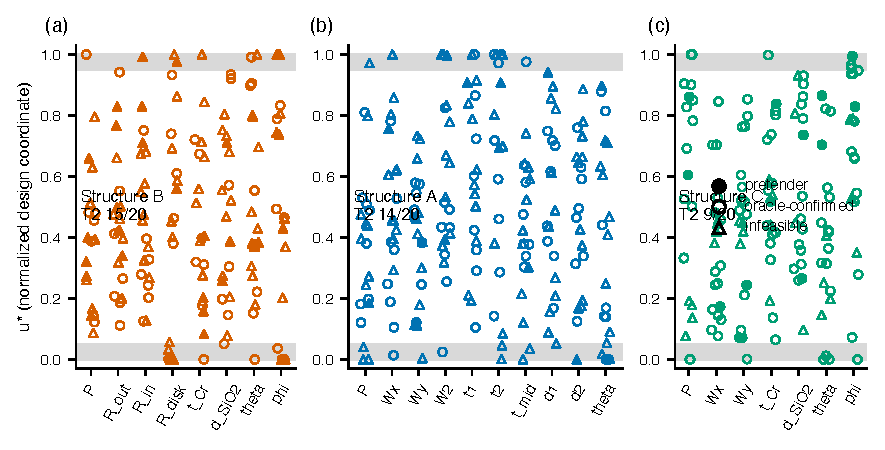
\includegraphics{figures/figS1_box_edge_geometry.pdf}
\caption{Per-parameter position of every committed geometry inside the design box (seed 42; one column per design parameter, y = the normalized coordinate u*). Grey bands mark the T2 box-edge region, within 0.05 of either bound. Filled markers are pretenders and open markers oracle-confirmed designs; triangles are geometries that violate a generator constraint. The in-band counts equal the T2 totals of Supplementary Table S1.}
\label{fig:S1}
\end{figure}

\begin{figure}[htbp]
\centering
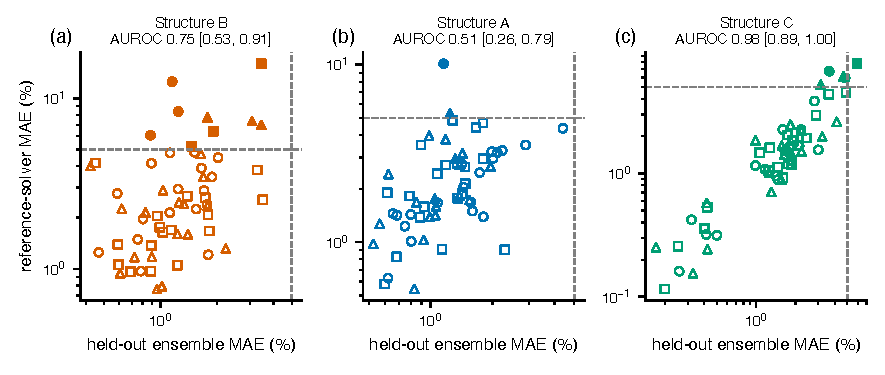
\includegraphics{figures/figS2_heldout_vs_rcwa.pdf}
\caption{Held-out ensemble error against reference-solver error for every valid committed geometry, per structure and training seed (log-log). The held-out ensemble error is the mean absolute error of the two surrogates that did \emph{not} commit the design, so it is available without any solver call. Dashed lines mark tau = 5 \%; filled markers are pretenders. Panel titles give the pooled AUROC for separating pretenders from oracle-confirmed designs, with its bootstrap 95 \% interval.}
\label{fig:S2}
\end{figure}

\section*{S8. The as-submitted arm of Section 3.10}

The identical protocol run end to end on the release of \cite{choi20261} that the published pipeline superseded (upstream commit \texttt{920b1bd}; fixed Fourier order 5, complex128; datasets struct\_A\_vis\_500 (479 good, 380--780 nm), struct\_B\_500 (461, 400--1800 nm), struct\_C\_500 (400, 400--1800 nm); C trained on 300 samples with a {[}50, 400{]} nm normalization box and 13 physics features). Artifacts: \texttt{results\_v8/}. The tables below are the S1, S2 and S6 equivalents for that arm.

\subsection*{S8.1. Per-run reliability accounting (as-submitted arm)}

\begin{landscape}
\begingroup
\setlength{\tabcolsep}{2pt}\tiny
\captionof{table}{S8. The as-submitted arm of Section 3.10}
\label{tab:8}
{\def\LTcaptype{none} % do not increment counter
\begin{longtable}[]{@{}lllllllllllllllll@{}}
\toprule\noalign{}
S & seed & n\_valid & surrogate-claimed {[}Wilson 95 \%{]} & oracle-confirmed {[}Wilson{]} & pretenders {[}Wilson{]} & \ensuremath{\Delta}-flagged {[}Wilson{]} & flag thr (\%) & modes & T1 & T2 & T3 & T4 & tail RSD & endpoint spread (u) & \ensuremath{\rho}(RCWA, Surr) {[}CI95{]} & p \\
\midrule\noalign{}
\endhead
\bottomrule\noalign{}
\endlastfoot
A & 42 & 20 & 20 {[}83.9, 100.0{]} & 11 {[}34.2, 74.2{]} & 9 {[}25.8, 65.8{]} & 0 {[}0.0, 16.1{]} & 9.69 & 20 & 19 & 15 & 0 & 0 & 0.0175 & 1.978 & +0.18 {[}-0.28, 0.58{]} & 0.435 \\
A & 123 & 20 & 20 {[}83.9, 100.0{]} & 11 {[}34.2, 74.2{]} & 9 {[}25.8, 65.8{]} & 1 {[}0.9, 23.6{]} & 9.68 & 18 & 19 & 16 & 3 & 0 & 0.0257 & 1.98 & +0.39 {[}-0.08, 0.72{]} & 0.086 \\
A & 777 & 20 & 20 {[}83.9, 100.0{]} & 11 {[}34.2, 74.2{]} & 9 {[}25.8, 65.8{]} & 1 {[}0.9, 23.6{]} & 9.46 & 19 & 20 & 16 & 2 & 0 & 0.0138 & 2.019 & +0.45 {[}-0.02, 0.75{]} & 0.048 \\
B & 42 & 20 & 20 {[}83.9, 100.0{]} & 11 {[}34.2, 74.2{]} & 9 {[}25.8, 65.8{]} & 6 {[}14.5, 51.9{]} & 6.37 & 17 & 16 & 14 & 5 & 0 & 0.0127 & 1.64 & -0.03 {[}-0.47, 0.42{]} & 0.890 \\
B & 123 & 20 & 20 {[}83.9, 100.0{]} & 9 {[}25.8, 65.8{]} & 11 {[}34.2, 74.2{]} & 8 {[}21.9, 61.3{]} & 6.52 & 18 & 20 & 16 & 4 & 0 & 0.0084 & 1.643 & -0.11 {[}-0.53, 0.35{]} & 0.654 \\
B & 777 & 20 & 20 {[}83.9, 100.0{]} & 10 {[}29.9, 70.1{]} & 10 {[}29.9, 70.1{]} & 6 {[}14.5, 51.9{]} & 6.56 & 15 & 18 & 14 & 7 & 0 & 0.0239 & 1.69 & +0.20 {[}-0.27, 0.60{]} & 0.391 \\
C & 42 & 20 & 20 {[}83.9, 100.0{]} & 7 {[}18.1, 56.7{]} & 13 {[}43.3, 81.9{]} & 3 {[}5.2, 36.0{]} & 7.73 & 15 & 11 & 11 & 7 & 0 & 0.0171 & 1.62 & -0.04 {[}-0.47, 0.41{]} & 0.880 \\
C & 123 & 20 & 20 {[}83.9, 100.0{]} & 8 {[}21.9, 61.3{]} & 12 {[}38.7, 78.1{]} & 2 {[}2.8, 30.1{]} & 7.66 & 13 & 11 & 12 & 10 & 0 & 0.0145 & 1.624 & +0.53 {[}0.08, 0.80{]} & 0.016 \\
C & 777 & 19 & 19 {[}83.2, 100.0{]} & 6 {[}15.4, 54.0{]} & 13 {[}46.0, 84.6{]} & 2 {[}2.9, 31.4{]} & 8.0 & 15 & 11 & 12 & 7 & 0 & 0.0021 & 1.676 & +0.28 {[}-0.21, 0.65{]} & 0.254 \\
\textbf{all} & & 179 & & & \textbf{95/179} (A 27/60, B 30/60, C 38/59) & & & & & & & & & & & \\
\end{longtable}
}
\endgroup
\end{landscape}

\subsection*{S8.2. Commitment-rule comparison (seed 42; as-submitted arm)}

\begin{landscape}
\begingroup
\setlength{\tabcolsep}{2pt}\tiny
\captionof{table}{S8. The as-submitted arm of Section 3.10}
\label{tab:9}
{\def\LTcaptype{none} % do not increment counter
\begin{longtable}[]{@{}lllllllll@{}}
\toprule\noalign{}
S & rule & surrogate-claimed & oracle-confirmed & pretenders (of n) & pretenders / claimed {[}Wilson{]} & mean oracle MAE (\%) & Fisher p vs best-of-8 (design-level) & Fisher p (conditional on claimed) \\
\midrule\noalign{}
\endhead
\bottomrule\noalign{}
\endlastfoot
A & gradient best-of-8 & 20 & 11 & 9/20 & 9/20 {[}25.8, 65.8{]} & 4.85 & --- & --- \\
A & random search (budget-matched) & 19 & 9 & 10/20 & 10/19 {[}31.7, 72.7{]} & 5.45 & 1.000 & 0.752 \\
A & single start (mid-box) & 20 & 12 & 8/20 & 8/20 {[}21.9, 61.3{]} & 5.49 & 1.000 & 1.000 \\
B & gradient best-of-8 & 20 & 11 & 9/20 & 9/20 {[}25.8, 65.8{]} & 6.65 & --- & --- \\
B & random search (budget-matched) & 19 & 5 & 14/20 & 14/19 {[}51.2, 88.2{]} & 10.79 & 0.200 & 0.105 \\
B & single start (mid-box) & 20 & 11 & 9/20 & 9/20 {[}25.8, 65.8{]} & 5.96 & 1.000 & 1.000 \\
C & gradient best-of-8 & 20 & 7 & 13/20 & 13/20 {[}43.3, 81.9{]} & 6.85 & --- & --- \\
C & random search (budget-matched) & 16 & 0 & 16/20 & 16/16 {[}80.6, 100.0{]} & 9.17 & 0.480 & 0.011 \\
C & single start (mid-box) & 17 & 8 & 9/20 & 9/17 {[}31.0, 73.8{]} & 7.18 & 0.341 & 0.516 \\
\end{longtable}
}
\endgroup
\end{landscape}

\subsection*{S8.3. Per-design table (as-submitted arm)}

Source: \texttt{results\_v8/} (reliability, recoverability JSONs; rcwa npz). \ensuremath{\tau} = 5 \%. status: pretender = Surr \ensuremath{\leq} \ensuremath{\tau} \& RCWA \textgreater{} \ensuremath{\tau}; confirmed = both \ensuremath{\leq} \ensuremath{\tau}; honest-failure = Surr \textgreater{} \ensuremath{\tau}; degenerate = solver failure.

\begingroup
\setlength{\tabcolsep}{2pt}\tiny
\captionof{table}{S8. The as-submitted arm of Section 3.10}
\label{tab:10}
{\def\LTcaptype{none} % do not increment counter
\begin{longtable}[]{@{}lllllllllllllllll@{}}
\toprule\noalign{}
S & seed & \# & idx & Surr MAE \% & RCWA MAE \% & \ensuremath{\Delta} pp & status & T1 & T2 & T3 & T4 & Surr@truth \% & \ensuremath{\|}u*\ensuremath{-}u\_true\ensuremath{\|} & support viol. & peak shift nm & peak \ensuremath{\Delta}A \\
\midrule\noalign{}
\endhead
\bottomrule\noalign{}
\endlastfoot
A & 42 & 1 & 190 & 0.07 & 1.74 & +1.67 & confirmed & 1 & 1 & 0 & 0 & 2.73 & 1.15 & 0 & +0 & -0.01 \\
A & 42 & 2 & 381 & 0.56 & 2.84 & +2.28 & confirmed & 1 & 1 & 0 & 0 & 4.01 & 1.15 & 0 & -12 & +0.02 \\
A & 42 & 3 & 451 & 1.22 & 2.74 & +1.52 & confirmed & 0 & 1 & 0 & 0 & 5.13 & 1.01 & 0 & +12 & -0.01 \\
A & 42 & 4 & 456 & 0.05 & 2.54 & +2.49 & confirmed & 1 & 1 & 0 & 0 & 0.66 & 1.47 & 1 & +0 & +0.00 \\
A & 42 & 5 & 482 & 0.17 & 7.56 & +7.38 & pretender & 1 & 1 & 0 & 0 & 2.72 & 1.12 & 1 & +109 & +0.11 \\
A & 42 & 6 & 24 & 0.47 & 7.42 & +6.95 & pretender & 1 & 1 & 0 & 0 & 5.83 & 0.75 & 0 & -48 & +0.18 \\
A & 42 & 7 & 16 & 0.47 & 3.26 & +2.79 & confirmed & 1 & 1 & 0 & 0 & 9.79 & 1.43 & 1 & +4 & +0.10 \\
A & 42 & 8 & 289 & 0.27 & 2.90 & +2.64 & confirmed & 1 & 0 & 0 & 0 & 2.65 & 1.24 & 0 & +4 & +0.02 \\
A & 42 & 9 & 327 & 0.21 & 5.83 & +5.62 & pretender & 1 & 1 & 0 & 0 & 6.77 & 1.41 & 1 & -28 & +0.01 \\
A & 42 & 10 & 101 & 0.63 & 6.76 & +6.13 & pretender & 1 & 1 & 0 & 0 & 4.37 & 1.66 & 0 & +323 & +0.03 \\
A & 42 & 11 & 249 & 1.24 & 4.44 & +3.19 & confirmed & 1 & 1 & 0 & 0 & 7.54 & 1.11 & 0 & -24 & -0.01 \\
A & 42 & 12 & 25 & 0.45 & 3.06 & +2.61 & confirmed & 1 & 0 & 0 & 0 & 5.14 & 0.74 & 0 & +12 & +0.08 \\
A & 42 & 13 & 37 & 1.00 & 4.26 & +3.26 & confirmed & 1 & 0 & 0 & 0 & 4.21 & 1.36 & 1 & -16 & -0.02 \\
A & 42 & 14 & 481 & 0.21 & 6.50 & +6.29 & pretender & 1 & 1 & 0 & 0 & 6.22 & 1.18 & 1 & +61 & +0.12 \\
A & 42 & 15 & 246 & 1.43 & 6.48 & +5.05 & pretender & 1 & 1 & 0 & 0 & 5.36 & 0.78 & 0 & +20 & -0.02 \\
A & 42 & 16 & 43 & 0.37 & 6.73 & +6.36 & pretender & 1 & 1 & 0 & 0 & 3.20 & 0.99 & 1 & +28 & +0.12 \\
A & 42 & 17 & 333 & 0.60 & 4.22 & +3.63 & confirmed & 1 & 0 & 0 & 0 & 5.10 & 1.08 & 0 & +20 & +0.06 \\
A & 42 & 18 & 312 & 1.46 & 7.36 & +5.90 & pretender & 1 & 0 & 0 & 0 & 6.63 & 0.74 & 1 & -16 & +0.15 \\
A & 42 & 19 & 6 & 0.20 & 5.92 & +5.72 & pretender & 1 & 1 & 0 & 0 & 4.44 & 0.92 & 1 & -4 & +0.12 \\
A & 42 & 20 & 413 & 0.08 & 4.36 & +4.28 & confirmed & 1 & 1 & 0 & 0 & 0.96 & 1.39 & 1 & +0 & +0.04 \\
A & 123 & 1 & 190 & 0.04 & 2.14 & +2.10 & confirmed & 1 & 1 & 0 & 0 & 3.85 & 0.99 & 0 & +0 & -0.01 \\
A & 123 & 2 & 381 & 0.73 & 4.04 & +3.31 & confirmed & 1 & 1 & 0 & 0 & 4.83 & 1.45 & 0 & +0 & +0.05 \\
A & 123 & 3 & 451 & 1.04 & 4.60 & +3.56 & confirmed & 1 & 1 & 0 & 0 & 5.79 & 0.73 & 1 & +12 & +0.02 \\
A & 123 & 4 & 456 & 0.06 & 10.08 & +10.02 & pretender & 1 & 1 & 0 & 0 & 0.61 & 1.33 & 1 & +77 & +0.31 \\
A & 123 & 5 & 482 & 0.10 & 4.37 & +4.27 & confirmed & 1 & 1 & 0 & 0 & 3.12 & 1.45 & 1 & +0 & -0.03 \\
A & 123 & 6 & 24 & 0.31 & 8.76 & +8.45 & pretender & 1 & 1 & 0 & 0 & 6.51 & 1.10 & 0 & -81 & +0.14 \\
A & 123 & 7 & 16 & 0.50 & 7.13 & +6.63 & pretender & 1 & 1 & 0 & 0 & 9.40 & 1.65 & 0 & -97 & -0.01 \\
A & 123 & 8 & 289 & 0.32 & 3.97 & +3.65 & confirmed & 1 & 1 & 1 & 0 & 3.49 & 1.07 & 0 & -8 & +0.03 \\
A & 123 & 9 & 327 & 0.52 & 5.81 & +5.29 & pretender & 1 & 1 & 0 & 0 & 7.09 & 1.39 & 0 & -28 & -0.08 \\
A & 123 & 10 & 101 & 0.53 & 3.98 & +3.45 & confirmed & 1 & 1 & 0 & 0 & 2.21 & 1.61 & 1 & +8 & +0.11 \\
A & 123 & 11 & 249 & 0.57 & 4.65 & +4.08 & confirmed & 1 & 0 & 0 & 0 & 5.47 & 0.56 & 0 & -8 & -0.01 \\
A & 123 & 12 & 25 & 0.39 & 9.12 & +8.73 & pretender & 1 & 0 & 1 & 0 & 4.30 & 1.17 & 0 & -20 & +0.04 \\
A & 123 & 13 & 37 & 0.75 & 7.94 & +7.19 & pretender & 1 & 0 & 0 & 0 & 4.96 & 1.38 & 1 & +12 & +0.06 \\
A & 123 & 14 & 481 & 0.25 & 3.50 & +3.25 & confirmed & 1 & 1 & 0 & 0 & 6.43 & 0.95 & 1 & -12 & +0.03 \\
A & 123 & 15 & 246 & 2.63 & 6.81 & +4.18 & pretender & 0 & 1 & 0 & 0 & 4.44 & 0.50 & 0 & +32 & +0.05 \\
A & 123 & 16 & 43 & 0.24 & 2.82 & +2.59 & confirmed & 1 & 1 & 0 & 0 & 3.34 & 0.90 & 0 & -8 & +0.03 \\
A & 123 & 17 & 333 & 0.65 & 8.08 & +7.42 & pretender & 1 & 0 & 1 & 0 & 3.18 & 0.96 & 0 & +36 & -0.02 \\
A & 123 & 18 & 312 & 2.33 & 9.62 & +7.29 & pretender & 1 & 1 & 0 & 0 & 8.95 & 0.74 & 1 & -24 & +0.13 \\
A & 123 & 19 & 6 & 0.11 & 3.17 & +3.06 & confirmed & 1 & 1 & 0 & 0 & 10.10 & 0.99 & 0 & -32 & -0.00 \\
A & 123 & 20 & 413 & 0.06 & 4.26 & +4.20 & confirmed & 1 & 1 & 0 & 0 & 0.54 & 1.52 & 0 & +0 & -0.05 \\
A & 777 & 1 & 190 & 0.10 & 1.65 & +1.55 & confirmed & 1 & 0 & 1 & 0 & 1.36 & 1.49 & 1 & +0 & -0.01 \\
A & 777 & 2 & 381 & 0.64 & 4.80 & +4.16 & confirmed & 1 & 1 & 0 & 0 & 2.92 & 1.08 & 1 & +0 & +0.02 \\
A & 777 & 3 & 451 & 0.79 & 4.04 & +3.25 & confirmed & 1 & 0 & 0 & 0 & 5.63 & 1.00 & 0 & +12 & -0.00 \\
A & 777 & 4 & 456 & 0.05 & 3.82 & +3.77 & confirmed & 1 & 1 & 0 & 0 & 1.85 & 0.83 & 0 & +0 & -0.03 \\
A & 777 & 5 & 482 & 0.12 & 4.63 & +4.51 & confirmed & 1 & 1 & 0 & 0 & 0.70 & 1.61 & 0 & +0 & -0.03 \\
A & 777 & 6 & 24 & 0.39 & 3.96 & +3.57 & confirmed & 1 & 1 & 0 & 0 & 4.57 & 0.93 & 0 & -28 & +0.08 \\
A & 777 & 7 & 16 & 0.48 & 4.73 & +4.25 & confirmed & 1 & 0 & 0 & 0 & 9.69 & 1.17 & 0 & +4 & -0.09 \\
A & 777 & 8 & 289 & 0.33 & 6.11 & +5.77 & pretender & 1 & 1 & 0 & 0 & 2.81 & 1.04 & 0 & -20 & -0.02 \\
A & 777 & 9 & 327 & 0.47 & 6.63 & +6.16 & pretender & 1 & 1 & 0 & 0 & 6.93 & 1.26 & 1 & -24 & +0.01 \\
A & 777 & 10 & 101 & 0.64 & 11.17 & +10.52 & pretender & 1 & 1 & 0 & 0 & 3.73 & 1.11 & 0 & +186 & +0.11 \\
A & 777 & 11 & 249 & 0.68 & 7.44 & +6.76 & pretender & 1 & 1 & 0 & 0 & 6.71 & 0.71 & 0 & +44 & -0.05 \\
A & 777 & 12 & 25 & 0.25 & 6.63 & +6.37 & pretender & 1 & 1 & 0 & 0 & 6.24 & 1.18 & 0 & +40 & +0.06 \\
A & 777 & 13 & 37 & 0.75 & 2.58 & +1.83 & confirmed & 1 & 1 & 0 & 0 & 4.63 & 1.41 & 0 & -4 & +0.02 \\
A & 777 & 14 & 481 & 0.14 & 1.97 & +1.83 & confirmed & 1 & 0 & 0 & 0 & 6.49 & 0.40 & 0 & -12 & -0.04 \\
A & 777 & 15 & 246 & 0.69 & 9.73 & +9.04 & pretender & 1 & 1 & 0 & 0 & 4.97 & 1.07 & 0 & -283 & -0.02 \\
A & 777 & 16 & 43 & 0.16 & 4.39 & +4.23 & confirmed & 1 & 1 & 0 & 0 & 3.93 & 1.14 & 0 & +44 & +0.02 \\
A & 777 & 17 & 333 & 0.51 & 7.36 & +6.85 & pretender & 1 & 1 & 0 & 0 & 2.69 & 1.33 & 0 & +48 & +0.07 \\
A & 777 & 18 & 312 & 1.48 & 5.32 & +3.84 & pretender & 1 & 1 & 0 & 0 & 7.92 & 1.18 & 0 & -81 & -0.10 \\
A & 777 & 19 & 6 & 0.71 & 5.21 & +4.50 & pretender & 1 & 1 & 0 & 0 & 9.07 & 1.21 & 0 & +0 & -0.00 \\
A & 777 & 20 & 413 & 0.07 & 3.36 & +3.29 & confirmed & 1 & 1 & 1 & 0 & 0.76 & 1.04 & 0 & +0 & -0.03 \\
B & 42 & 1 & 358 & 0.45 & 1.84 & +1.38 & confirmed & 1 & 0 & 1 & 0 & 3.65 & 0.63 & 0 & +28 & -0.03 \\
B & 42 & 2 & 43 & 1.14 & 2.60 & +1.46 & confirmed & 0 & 1 & 0 & 0 & 3.06 & 0.37 & 0 & +14 & +0.02 \\
B & 42 & 3 & 24 & 0.76 & 3.80 & +3.05 & confirmed & 1 & 0 & 1 & 0 & 3.14 & 0.59 & 0 & +28 & -0.02 \\
B & 42 & 4 & 428 & 0.43 & 3.76 & +3.33 & confirmed & 1 & 1 & 0 & 0 & 2.87 & 0.78 & 0 & +71 & +0.04 \\
B & 42 & 5 & 487 & 1.07 & 1.96 & +0.88 & confirmed & 0 & 0 & 0 & 0 & 1.66 & 0.21 & 0 & +0 & +0.00 \\
B & 42 & 6 & 396 & 1.10 & 1.62 & +0.52 & confirmed & 0 & 1 & 0 & 0 & 2.93 & 0.26 & 0 & +14 & -0.03 \\
B & 42 & 7 & 302 & 0.61 & 31.64 & +31.03 & pretender & 1 & 1 & 0 & 0 & 6.10 & 1.20 & 1 & +933 & +0.29 \\
B & 42 & 8 & 468 & 0.63 & 5.86 & +5.23 & pretender & 1 & 1 & 0 & 0 & 3.90 & 0.66 & 0 & -339 & -0.03 \\
B & 42 & 9 & 310 & 0.70 & 2.78 & +2.08 & confirmed & 1 & 1 & 0 & 0 & 3.09 & 0.74 & 0 & +57 & -0.01 \\
B & 42 & 10 & 38 & 1.88 & 6.82 & +4.95 & pretender & 1 & 1 & 0 & 0 & 7.98 & 0.50 & 0 & +14 & +0.10 \\
B & 42 & 11 & 16 & 1.03 & 2.51 & +1.48 & confirmed & 0 & 1 & 0 & 0 & 2.71 & 0.39 & 0 & +28 & -0.01 \\
B & 42 & 12 & 168 & 0.35 & 7.58 & +7.23 & pretender & 1 & 1 & 1 & 0 & 2.17 & 0.87 & 0 & -57 & -0.07 \\
B & 42 & 13 & 339 & 0.30 & 2.56 & +2.25 & confirmed & 1 & 0 & 0 & 0 & 3.39 & 0.60 & 0 & +42 & -0.04 \\
B & 42 & 14 & 146 & 0.30 & 7.54 & +7.24 & pretender & 1 & 0 & 0 & 0 & 1.89 & 0.46 & 0 & +28 & -0.09 \\
B & 42 & 15 & 118 & 0.31 & 1.49 & +1.18 & confirmed & 1 & 0 & 1 & 0 & 4.22 & 0.73 & 0 & -28 & +0.04 \\
B & 42 & 16 & 481 & 1.22 & 7.25 & +6.03 & pretender & 1 & 1 & 0 & 0 & 4.92 & 0.64 & 0 & +71 & +0.02 \\
B & 42 & 17 & 172 & 0.37 & 10.74 & +10.37 & pretender & 1 & 1 & 0 & 0 & 4.17 & 0.48 & 0 & +438 & +0.21 \\
B & 42 & 18 & 311 & 0.67 & 13.40 & +12.72 & pretender & 1 & 1 & 1 & 0 & 2.77 & 0.34 & 0 & -820 & -0.06 \\
B & 42 & 19 & 51 & 0.49 & 3.53 & +3.04 & confirmed & 1 & 1 & 0 & 0 & 1.81 & 0.71 & 0 & +0 & -0.08 \\
B & 42 & 20 & 255 & 1.07 & 13.68 & +12.61 & pretender & 1 & 1 & 0 & 0 & 1.59 & 1.68 & 0 & +0 & +0.18 \\
B & 123 & 1 & 358 & 0.65 & 7.31 & +6.66 & pretender & 1 & 0 & 1 & 0 & 4.04 & 0.85 & 0 & -71 & +0.00 \\
B & 123 & 2 & 43 & 0.97 & 4.53 & +3.56 & confirmed & 1 & 1 & 0 & 0 & 3.53 & 0.45 & 0 & +28 & +0.02 \\
B & 123 & 3 & 24 & 0.47 & 3.77 & +3.31 & confirmed & 1 & 0 & 1 & 0 & 2.45 & 0.45 & 0 & +42 & +0.01 \\
B & 123 & 4 & 428 & 0.56 & 3.50 & +2.94 & confirmed & 1 & 1 & 0 & 0 & 3.27 & 0.51 & 0 & -14 & +0.04 \\
B & 123 & 5 & 487 & 1.15 & 3.89 & +2.74 & confirmed & 1 & 1 & 0 & 0 & 1.36 & 0.35 & 0 & -99 & -0.00 \\
B & 123 & 6 & 396 & 0.90 & 2.91 & +2.01 & confirmed & 1 & 0 & 1 & 0 & 2.58 & 0.52 & 0 & +99 & -0.03 \\
B & 123 & 7 & 302 & 0.56 & 16.43 & +15.87 & pretender & 1 & 1 & 0 & 0 & 5.42 & 1.21 & 1 & +749 & +0.11 \\
B & 123 & 8 & 468 & 0.39 & 10.68 & +10.29 & pretender & 1 & 1 & 0 & 0 & 6.64 & 1.14 & 0 & +424 & +0.21 \\
B & 123 & 9 & 310 & 0.61 & 3.07 & +2.46 & confirmed & 1 & 1 & 0 & 0 & 2.19 & 0.88 & 0 & -14 & -0.02 \\
B & 123 & 10 & 38 & 1.36 & 5.35 & +3.99 & pretender & 1 & 1 & 0 & 0 & 10.67 & 0.83 & 0 & -57 & +0.05 \\
B & 123 & 11 & 16 & 0.90 & 6.87 & +5.97 & pretender & 1 & 1 & 0 & 0 & 2.85 & 0.43 & 0 & +0 & -0.04 \\
B & 123 & 12 & 168 & 0.59 & 25.79 & +25.20 & pretender & 1 & 1 & 0 & 0 & 2.59 & 1.24 & 0 & -156 & -0.19 \\
B & 123 & 13 & 339 & 0.32 & 3.75 & +3.43 & confirmed & 1 & 0 & 0 & 0 & 1.99 & 0.64 & 0 & +0 & -0.06 \\
B & 123 & 14 & 146 & 0.30 & 9.42 & +9.12 & pretender & 1 & 1 & 0 & 0 & 1.05 & 0.90 & 0 & +57 & -0.12 \\
B & 123 & 15 & 118 & 0.34 & 26.96 & +26.62 & pretender & 1 & 1 & 1 & 0 & 3.04 & 1.06 & 0 & -636 & -0.30 \\
B & 123 & 16 & 481 & 1.12 & 4.50 & +3.38 & confirmed & 1 & 1 & 0 & 0 & 5.59 & 0.45 & 0 & +57 & +0.08 \\
B & 123 & 17 & 172 & 0.42 & 10.17 & +9.74 & pretender & 1 & 1 & 0 & 0 & 2.45 & 0.41 & 0 & +537 & +0.13 \\
B & 123 & 18 & 311 & 1.02 & 5.51 & +4.50 & pretender & 1 & 1 & 0 & 0 & 5.03 & 1.26 & 0 & -552 & +0.13 \\
B & 123 & 19 & 51 & 0.53 & 2.01 & +1.47 & confirmed & 1 & 1 & 0 & 0 & 2.68 & 0.72 & 0 & -14 & -0.01 \\
B & 123 & 20 & 255 & 1.47 & 17.50 & +16.03 & pretender & 1 & 1 & 0 & 0 & 2.70 & 1.37 & 0 & -57 & +0.14 \\
B & 777 & 1 & 358 & 0.64 & 1.69 & +1.05 & confirmed & 0 & 0 & 1 & 0 & 3.99 & 0.75 & 0 & -14 & -0.02 \\
B & 777 & 2 & 43 & 1.00 & 2.08 & +1.07 & confirmed & 0 & 1 & 1 & 0 & 4.39 & 0.41 & 0 & +14 & -0.01 \\
B & 777 & 3 & 24 & 0.45 & 2.56 & +2.11 & confirmed & 1 & 0 & 1 & 0 & 3.07 & 0.73 & 0 & +0 & +0.01 \\
B & 777 & 4 & 428 & 0.42 & 4.07 & +3.66 & confirmed & 1 & 1 & 0 & 0 & 2.90 & 0.64 & 0 & +0 & +0.03 \\
B & 777 & 5 & 487 & 1.26 & 4.44 & +3.18 & confirmed & 1 & 0 & 1 & 0 & 2.08 & 0.27 & 0 & -113 & -0.00 \\
B & 777 & 6 & 396 & 1.00 & 3.16 & +2.16 & confirmed & 1 & 0 & 1 & 0 & 2.57 & 0.21 & 0 & +0 & +0.00 \\
B & 777 & 7 & 302 & 1.16 & 12.76 & +11.60 & pretender & 1 & 1 & 0 & 0 & 4.89 & 1.31 & 1 & +0 & +0.10 \\
B & 777 & 8 & 468 & 0.79 & 12.28 & +11.48 & pretender & 1 & 0 & 1 & 0 & 6.12 & 1.03 & 0 & -665 & -0.10 \\
B & 777 & 9 & 310 & 0.71 & 2.16 & +1.45 & confirmed & 1 & 1 & 0 & 0 & 2.22 & 0.79 & 0 & -14 & -0.02 \\
B & 777 & 10 & 38 & 1.61 & 7.03 & +5.42 & pretender & 1 & 1 & 0 & 0 & 9.30 & 0.78 & 1 & +28 & -0.02 \\
B & 777 & 11 & 16 & 0.86 & 6.27 & +5.42 & pretender & 1 & 1 & 1 & 0 & 3.27 & 0.45 & 0 & +0 & -0.07 \\
B & 777 & 12 & 168 & 0.24 & 5.52 & +5.28 & pretender & 1 & 0 & 0 & 0 & 2.63 & 0.79 & 0 & +1089 & +0.00 \\
B & 777 & 13 & 339 & 0.30 & 4.49 & +4.19 & confirmed & 1 & 1 & 0 & 0 & 1.68 & 0.53 & 0 & -14 & -0.06 \\
B & 777 & 14 & 146 & 0.25 & 5.16 & +4.91 & pretender & 1 & 1 & 0 & 0 & 1.63 & 0.50 & 0 & +99 & -0.04 \\
B & 777 & 15 & 118 & 0.51 & 33.58 & +33.07 & pretender & 1 & 1 & 0 & 0 & 4.00 & 1.22 & 0 & -42 & -0.36 \\
B & 777 & 16 & 481 & 1.13 & 4.96 & +3.82 & confirmed & 1 & 1 & 0 & 0 & 5.83 & 0.59 & 0 & +71 & +0.09 \\
B & 777 & 17 & 172 & 0.34 & 4.64 & +4.29 & confirmed & 1 & 1 & 0 & 0 & 3.21 & 0.91 & 0 & -42 & +0.06 \\
B & 777 & 18 & 311 & 1.11 & 9.27 & +8.16 & pretender & 1 & 1 & 0 & 0 & 5.04 & 1.43 & 0 & -834 & -0.06 \\
B & 777 & 19 & 51 & 0.80 & 21.24 & +20.44 & pretender & 1 & 1 & 0 & 0 & 2.43 & 0.80 & 1 & +14 & -0.32 \\
B & 777 & 20 & 255 & 1.02 & 13.14 & +12.13 & pretender & 1 & 1 & 0 & 0 & 1.82 & 1.41 & 0 & +1343 & +0.22 \\
C & 42 & 1 & 363 & 2.57 & 9.15 & +6.58 & pretender & 1 & 1 & 0 & 0 & 5.92 & 0.84 & 1 & +14/-255 & +0.54/+0.05 \\
C & 42 & 2 & 221 & 0.50 & 3.60 & +3.10 & confirmed & 1 & 0 & 1 & 0 & 2.59 & 0.76 & 0 & +127/+42 & +0.07/+0.02 \\
C & 42 & 3 & 399 & 2.16 & 3.79 & +1.63 & confirmed & 0 & 0 & 1 & 0 & 6.11 & 0.63 & 0 & -99/+0 & +0.08/+0.01 \\
C & 42 & 4 & 382 & 1.75 & 3.42 & +1.67 & confirmed & 0 & 0 & 0 & 0 & 2.61 & 0.18 & 0 & +14/+42 & -0.02/+0.00 \\
C & 42 & 5 & 121 & 1.09 & 3.37 & +2.28 & confirmed & 1 & 0 & 1 & 0 & 3.69 & 0.25 & 0 & +0/+156 & +0.04/+0.06 \\
C & 42 & 6 & 178 & 1.75 & 3.80 & +2.05 & confirmed & 0 & 0 & 0 & 0 & 2.63 & 0.46 & 0 & +0/+0 & +0.04/-0.00 \\
C & 42 & 7 & 203 & 3.88 & 5.59 & +1.71 & pretender & 0 & 0 & 1 & 0 & 9.29 & 0.42 & 0 & +382/+0 & +0.08/-0.01 \\
C & 42 & 8 & 341 & 0.42 & 5.72 & +5.30 & pretender & 1 & 0 & 1 & 0 & 1.10 & 0.11 & 0 & +113/-354 & +0.04/-0.11 \\
C & 42 & 9 & 139 & 1.36 & 6.87 & +5.51 & pretender & 1 & 1 & 0 & 0 & 2.41 & 0.28 & 1 & -113/+0 & +0.15/-0.02 \\
C & 42 & 10 & 244 & 3.29 & 6.49 & +3.20 & pretender & 0 & 1 & 0 & 0 & 5.70 & 0.69 & 0 & +127/+28 & +0.00/-0.10 \\
C & 42 & 11 & 176 & 3.88 & 11.06 & +7.18 & pretender & 0 & 1 & 0 & 0 & 2.56 & 0.94 & 0 & +42/+156 & +0.07/-0.19 \\
C & 42 & 12 & 271 & 0.83 & 5.67 & +4.84 & pretender & 1 & 0 & 1 & 0 & 3.32 & 0.50 & 0 & +1174/+0 & +0.11/+0.02 \\
C & 42 & 13 & 245 & 0.40 & 10.79 & +10.39 & pretender & 1 & 1 & 0 & 0 & 1.29 & 0.28 & 1 & +962/-410 & +0.34/-0.04 \\
C & 42 & 14 & 6 & 2.79 & 3.82 & +1.03 & confirmed & 0 & 1 & 0 & 0 & 3.93 & 0.18 & 0 & +226/-14 & -0.01/+0.01 \\
C & 42 & 15 & 208 & 0.87 & 14.54 & +13.67 & pretender & 1 & 1 & 0 & 0 & 2.14 & 0.33 & 0 & +848/-283 & +0.29/-0.12 \\
C & 42 & 16 & 129 & 2.01 & 3.99 & +1.98 & confirmed & 0 & 1 & 0 & 0 & 8.38 & 1.24 & 0 & -14/-127 & -0.02/-0.08 \\
C & 42 & 17 & 463 & 3.62 & 5.70 & +2.08 & pretender & 0 & 1 & 0 & 0 & 2.32 & 1.45 & 1 & +28/+156 & +0.00/-0.04 \\
C & 42 & 18 & 137 & 2.76 & 9.78 & +7.02 & pretender & 1 & 1 & 0 & 0 & 6.03 & 0.96 & 0 & -71/-28 & -0.07/-0.01 \\
C & 42 & 19 & 45 & 2.13 & 7.92 & +5.78 & pretender & 1 & 1 & 0 & 0 & 4.97 & 0.69 & 0 & +14/-42 & +0.03/+0.01 \\
C & 42 & 20 & 403 & 0.43 & 11.93 & +11.50 & pretender & 1 & 0 & 1 & 0 & 0.54 & 0.48 & 0 & +1400/+0 & +0.37/+0.00 \\
C & 123 & 1 & 363 & 2.40 & 9.22 & +6.82 & pretender & 1 & 1 & 1 & 0 & 4.50 & 0.73 & 1 & -14/-71 & +0.51/+0.09 \\
C & 123 & 2 & 221 & 0.47 & 3.50 & +3.02 & confirmed & 1 & 0 & 1 & 0 & 1.35 & 0.24 & 0 & -14/+85 & -0.02/+0.07 \\
C & 123 & 3 & 399 & 1.83 & 2.36 & +0.53 & confirmed & 0 & 0 & 1 & 0 & 4.87 & 0.43 & 0 & -57/+0 & +0.04/+0.05 \\
C & 123 & 4 & 382 & 1.70 & 3.66 & +1.96 & confirmed & 0 & 0 & 0 & 0 & 2.77 & 0.21 & 0 & -14/+57 & -0.02/+0.00 \\
C & 123 & 5 & 121 & 1.04 & 6.06 & +5.01 & pretender & 1 & 1 & 0 & 0 & 3.42 & 0.48 & 0 & +0/-608 & -0.03/-0.00 \\
C & 123 & 6 & 178 & 1.80 & 7.56 & +5.76 & pretender & 1 & 0 & 0 & 0 & 2.10 & 0.43 & 0 & +0/+14 & +0.07/-0.08 \\
C & 123 & 7 & 203 & 3.92 & 5.52 & +1.61 & pretender & 0 & 0 & 1 & 0 & 9.41 & 0.37 & 0 & +382/+0 & +0.14/-0.01 \\
C & 123 & 8 & 341 & 0.42 & 6.85 & +6.43 & pretender & 1 & 0 & 1 & 0 & 0.94 & 0.19 & 0 & -156/-99 & -0.08/-0.09 \\
C & 123 & 9 & 139 & 1.89 & 2.73 & +0.84 & confirmed & 0 & 1 & 0 & 0 & 2.41 & 0.79 & 0 & +42/+85 & -0.07/+0.04 \\
C & 123 & 10 & 244 & 4.06 & 8.89 & +4.84 & pretender & 0 & 1 & 0 & 0 & 6.51 & 1.10 & 0 & -834/-170 & -0.01/+0.05 \\
C & 123 & 11 & 176 & 3.13 & 8.02 & +4.89 & pretender & 0 & 1 & 1 & 0 & 2.44 & 1.22 & 0 & +368/-28 & -0.01/-0.24 \\
C & 123 & 12 & 271 & 0.73 & 4.54 & +3.81 & confirmed & 1 & 0 & 0 & 0 & 2.73 & 0.64 & 0 & +0/+1259 & +0.01/+0.03 \\
C & 123 & 13 & 245 & 0.37 & 5.56 & +5.19 & pretender & 1 & 0 & 1 & 0 & 2.20 & 1.09 & 1 & +424/-438 & +0.02/-0.06 \\
C & 123 & 14 & 6 & 3.32 & 3.67 & +0.36 & confirmed & 0 & 1 & 1 & 0 & 4.44 & 0.19 & 0 & +226/-28 & -0.00/+0.00 \\
C & 123 & 15 & 208 & 0.43 & 2.62 & +2.18 & confirmed & 1 & 1 & 1 & 0 & 2.31 & 0.39 & 0 & +42/-113 & +0.02/-0.03 \\
C & 123 & 16 & 129 & 2.72 & 7.82 & +5.10 & pretender & 0 & 1 & 0 & 0 & 7.89 & 1.25 & 0 & -71/+14 & -0.02/+0.16 \\
C & 123 & 17 & 463 & 4.20 & 14.46 & +10.26 & pretender & 1 & 1 & 0 & 0 & 3.62 & 1.52 & 1 & -339/+14 & +0.40/+0.26 \\
C & 123 & 18 & 137 & 3.60 & 6.80 & +3.20 & pretender & 0 & 1 & 0 & 0 & 5.62 & 0.86 & 0 & -28/-57 & -0.05/-0.01 \\
C & 123 & 19 & 45 & 2.49 & 11.26 & +8.77 & pretender & 1 & 1 & 0 & 0 & 5.38 & 0.74 & 0 & +71/-42 & +0.01/-0.01 \\
C & 123 & 20 & 403 & 0.42 & 2.38 & +1.96 & confirmed & 1 & 1 & 1 & 0 & 0.72 & 0.12 & 0 & +0/+0 & +0.02/+0.01 \\
C & 777 & 1 & 363 & 2.27 & 7.54 & +5.26 & pretender & 1 & 0 & 0 & 0 & 3.93 & 0.75 & 1 & -14/+0 & +0.46/+0.09 \\
C & 777 & 2 & 221 & 0.47 & 7.82 & +7.35 & pretender & 1 & 1 & 1 & 0 & 2.01 & 1.10 & 0 & +156/+170 & +0.10/+0.12 \\
C & 777 & 3 & 399 & 2.16 & 5.93 & +3.77 & pretender & 0 & 1 & 1 & 0 & 5.84 & 1.10 & 0 & -113/+0 & +0.00/-0.05 \\
C & 777 & 4 & 382 & 1.78 & 3.45 & +1.68 & confirmed & 0 & 0 & 0 & 0 & 3.09 & 0.19 & 0 & +42/+28 & +0.01/+0.00 \\
C & 777 & 5 & 121 & 1.20 & 4.52 & +3.32 & confirmed & 1 & 1 & 1 & 0 & 3.89 & 0.47 & 0 & +0/-622 & -0.03/-0.01 \\
C & 777 & 6 & 178 & 2.25 & 5.20 & +2.95 & pretender & 0 & 0 & 0 & 0 & 2.31 & 0.41 & 0 & +14/+0 & +0.02/+0.03 \\
C & 777 & 7 & 203 & 4.66 & 5.50 & +0.84 & pretender & 0 & 0 & 1 & 0 & 9.45 & 0.37 & 0 & +382/+0 & +0.10/-0.02 \\
C & 777 & 8 & 341 & 0.25 & 3.71 & +3.46 & confirmed & 1 & 0 & 1 & 0 & 0.81 & 0.05 & 0 & -156/+14 & -0.09/+0.01 \\
C & 777 & 9 & 139 & 1.53 & 5.08 & +3.55 & pretender & 1 & 1 & 0 & 0 & 2.86 & 0.62 & 0 & +14/+0 & -0.11/-0.05 \\
C & 777 & 10 & 244 & 4.07 & 5.81 & +1.73 & pretender & 0 & 0 & 0 & 0 & 6.92 & 0.72 & 0 & -566/+14 & -0.07/-0.06 \\
C & 777 & 11 & 176 & 2.69 & 5.12 & +2.42 & pretender & 0 & 1 & 0 & 0 & 1.95 & 0.91 & 0 & +42/+42 & +0.04/-0.28 \\
C & 777 & 12 & 271 & 0.84 & 3.70 & +2.86 & confirmed & 1 & 0 & 0 & 0 & 4.80 & 0.47 & 0 & +1061/+0 & +0.07/+0.01 \\
C & 777 & 13 & 245 & 0.48 & 8.85 & +8.37 & pretender & 1 & 1 & 0 & 0 & 1.73 & 0.76 & 1 & -71/-438 & +0.35/+0.05 \\
C & 777 & 14 & 6 & 2.35 & 3.84 & +1.49 & confirmed & 0 & 1 & 0 & 0 & 3.96 & 0.15 & 0 & +212/-28 & +0.01/+0.01 \\
C & 777 & 15 & 208 & 1.57 & 5.68 & +4.11 & pretender & 1 & 0 & 1 & 0 & 2.44 & 1.36 & 0 & +71/-297 & +0.17/+0.03 \\
C & 777 & 16 & 129 & 2.91 & --- & --- & degenerate & 0 & 1 & 0 & 0 & 8.84 & 1.16 & 0 & +nan/+nan & +nan/+nan \\
C & 777 & 17 & 463 & 3.47 & 5.08 & +1.61 & pretender & 0 & 1 & 1 & 0 & 2.10 & 1.42 & 0 & +42/+127 & -0.00/-0.03 \\
C & 777 & 18 & 137 & 3.13 & 10.87 & +7.75 & pretender & 1 & 1 & 0 & 0 & 5.61 & 1.36 & 1 & -71/-212 & +0.11/-0.04 \\
C & 777 & 19 & 45 & 1.90 & 11.37 & +9.46 & pretender & 1 & 1 & 0 & 0 & 4.63 & 0.76 & 0 & +57/-42 & +0.02/-0.01 \\
C & 777 & 20 & 403 & 0.43 & 2.60 & +2.16 & confirmed & 1 & 1 & 0 & 0 & 0.58 & 0.06 & 0 & +0/+0 & -0.01/+0.01 \\
\end{longtable}
}
\endgroup

Valid designs: 179; pretenders: 95.

\begin{thebibliography}{60}
\bibitem{choi20261}
S.-B. Choi, J. Kim, C.-M. Kang, "Physics-Based Transfer Learning for Neural Network Surrogates of Metal--Insulator--Metal Absorbers," \emph{Photonics and Nanostructures -- Fundamentals and Applications} \textbf{72}(Part B), 101617 (2026). doi:10.1016/j.photonics.2026.101617

\bibitem{landy20082}
N. I. Landy, S. Sajuyigbe, J. J. Mock, D. R. Smith, W. J. Padilla, "Perfect metamaterial absorber," \emph{Phys. Rev. Lett.} \textbf{100}, 207402 (2008). doi:10.1103/PhysRevLett.100.207402

\bibitem{ma20213}
W. Ma, Z. Liu, Z. A. Kudyshev, A. Boltasseva, W. Cai, Y. Liu, "Deep learning for the design of photonic structures," \emph{Nat. Photonics} \textbf{15}, 77--90 (2021). doi:10.1038/s41566-020-0685-y

\bibitem{jiang20214}
J. Jiang, M. Chen, J. A. Fan, "Deep neural networks for the evaluation and design of photonic devices," \emph{Nat. Rev. Mater.} \textbf{6}, 679--700 (2021). doi:10.1038/s41578-020-00260-1

\bibitem{wiecha20215}
P. R. Wiecha, A. Arbouet, C. Girard, O. L. Muskens, "Deep learning in nano-photonics: inverse design and beyond," \emph{Photonics Res.} \textbf{9}, B182 (2021). doi:10.1364/PRJ.415960

\bibitem{so20206}
S. So, T. Badloe, J. Noh, J. Bravo-Abad, J. Rho, "Deep learning enabled inverse design in nanophotonics," \emph{Nanophotonics} \textbf{9}, 1041--1057 (2020). doi:10.1515/nanoph-2019-0474

\bibitem{khairehwalieh20237}
A. Khaireh-Walieh, D. Langevin, P. Bennet, O. Teytaud, A. Moreau, P. R. Wiecha, "A newcomer\textquotesingle s guide to deep learning for inverse design in nano-photonics," \emph{Nanophotonics} \textbf{12}, 4387--4414 (2023). doi:10.1515/nanoph-2023-0527

\bibitem{qu20198}
Y. Qu, L. Jing, Y. Shen, M. Qiu, M. Solja\v{c}i\'c, "Migrating knowledge between physical scenarios based on artificial neural networks," \emph{ACS Photonics} \textbf{6}, 1168--1174 (2019). doi:10.1021/acsphotonics.8b01526

\bibitem{peng20249}
R. Peng, S. Ren, J. Malof, W. J. Padilla, "Transfer learning for metamaterial design and simulation," \emph{Nanophotonics} \textbf{13}, 2323--2334 (2024). doi:10.1515/nanoph-2023-0691

\bibitem{zhu202510}
L. Zhu, C. Lv, W. Hua, D. Huang, Y. Liu, "PTLOR-Net: physical transfer learning based optical response prediction network of metasurfaces," \emph{ACS Photonics} \textbf{12}, 2624--2636 (2025). doi:10.1021/acsphotonics.5c00104

\bibitem{kim202511}
G. Kim, J. Kim, "Efficient nanophotonic devices optimization using deep neural network trained with physics-based transfer learning methodology," \emph{Sci. Rep.} \textbf{15}, 39854 (2025). doi:10.1038/s41598-025-23519-5

\bibitem{zhang202312}
W. Zhang, L. Deng, L. Zhang, D. Wu, "A survey on negative transfer," \emph{IEEE/CAA J. Autom. Sinica} \textbf{10}, 305--329 (2023). doi:10.1109/JAS.2022.106004

\bibitem{kumar202013}
A. Kumar, S. Levine, "Model inversion networks for model-based optimization," \emph{NeurIPS} \textbf{33} (2020). arXiv:1912.13464

\bibitem{trabucco202114}
B. Trabucco, A. Kumar, X. Geng, S. Levine, "Conservative objective models for effective offline model-based optimization," \emph{ICML}, PMLR \textbf{139} (2021). arXiv:2107.06882

\bibitem{trabucco202215}
B. Trabucco, X. Geng, A. Kumar, S. Levine, "Design-Bench: benchmarks for data-driven offline model-based optimization," \emph{ICML}, PMLR \textbf{162} (2022). arXiv:2202.08450

\bibitem{fannjiang202016}
C. Fannjiang, J. Listgarten, "Autofocused oracles for model-based design," \emph{NeurIPS} \textbf{33} (2020). arXiv:2006.08052

\bibitem{alexandrov199817}
N. M. Alexandrov, J. E. Dennis, R. M. Lewis, V. Torczon, "A trust-region framework for managing the use of approximation models in optimization," \emph{Struct. Optim.} \textbf{15}, 16--23 (1998). doi:10.1007/BF01197433

\bibitem{booker199918}
A. J. Booker, J. E. Dennis, P. D. Frank, D. B. Serafini, V. Torczon, M. W. Trosset, "A rigorous framework for optimization of expensive functions by surrogates," \emph{Struct. Optim.} \textbf{17}, 1--13 (1999). doi:10.1007/BF01197708

\bibitem{forrester200919}
A. I. J. Forrester, A. J. Keane, "Recent advances in surrogate-based optimization," \emph{Prog. Aerosp. Sci.} \textbf{45}, 50--79 (2009). doi:10.1016/j.paerosci.2008.11.001

\bibitem{jin201120}
Y. Jin, "Surrogate-assisted evolutionary computation: recent advances and future challenges," \emph{Swarm Evol. Comput.} \textbf{1}, 61--70 (2011). doi:10.1016/j.swevo.2011.05.001

\bibitem{kennedy200021}
M. C. Kennedy, A. O\textquotesingle Hagan, "Predicting the output from a complex computer code when fast approximations are available," \emph{Biometrika} \textbf{87}, 1--13 (2000). doi:10.1093/biomet/87.1.1

\bibitem{peherstorfer201822}
B. Peherstorfer, K. Willcox, M. Gunzburger, "Survey of multifidelity methods in uncertainty propagation, inference, and optimization," \emph{SIAM Rev.} \textbf{60}, 550--591 (2018). doi:10.1137/16M1082469

\bibitem{meng202023}
X. Meng, G. E. Karniadakis, "A composite neural network that learns from multi-fidelity data," \emph{J. Comput. Phys.} \textbf{401}, 109020 (2020). doi:10.1016/j.jcp.2019.109020

\bibitem{brookes201924}
D. H. Brookes, H. Park, J. Listgarten, "Conditioning by adaptive sampling for robust design," \emph{ICML}, PMLR \textbf{97} (2019). arXiv:1901.10060

\bibitem{tripp202025}
A. Tripp, E. Daxberger, J. M. Hern\'andez-Lobato, "Sample-efficient optimization in the latent space of deep generative models via weighted retraining," \emph{NeurIPS} \textbf{33} (2020). arXiv:2006.09191

\bibitem{yu202126}
S. Yu, S. Ahn, L. Song, J. Shin, "RoMA: robust model adaptation for offline model-based optimization," \emph{NeurIPS} \textbf{34} (2021). arXiv:2110.14188

\bibitem{kim202527}
M. Kim, J. Gu, Y. Yuan, T. Yun et al., "Offline model-based optimization: comprehensive review," \emph{Trans. Mach. Learn. Res.} (2025). arXiv:2503.17286

\bibitem{manheim201828}
D. Manheim, S. Garrabrant, "Categorizing variants of Goodhart\textquotesingle s law" (2018). arXiv:1803.04585

\bibitem{skalse202229}
J. Skalse, N. H. R. Howe, D. Krasheninnikov, D. Krueger, "Defining and characterizing reward hacking," \emph{NeurIPS} \textbf{35} (2022). arXiv:2209.13085

\bibitem{gao202330}
L. Gao, J. Schulman, J. Hilton, "Scaling laws for reward model overoptimization," \emph{ICML}, PMLR \textbf{202} (2023). arXiv:2210.10760

\bibitem{surana202531}
S. Surana, N. Grinsztajn, T. Atkinson, P. Duckworth, T. D. Barrett, "Overconfident oracles: limitations of in silico sequence design benchmarking," \emph{ICML 2024 AI for Science Workshop} (2024). arXiv:2502.17246

\bibitem{pestourie202032}
R. Pestourie, Y. Mroueh, T. V. Nguyen, P. Das, S. G. Johnson, "Active learning of deep surrogates for PDEs: application to metasurface design," \emph{npj Comput. Mater.} \textbf{6}, 164 (2020). doi:10.1038/s41524-020-00431-2

\bibitem{jiang201933}
J. Jiang, J. A. Fan, "Global optimization of dielectric metasurfaces using a physics-driven neural network," \emph{Nano Lett.} \textbf{19}, 5366--5372 (2019). doi:10.1021/acs.nanolett.9b01857

\bibitem{nosek201834}
B. A. Nosek, C. R. Ebersole, A. C. DeHaven, D. T. Mellor, "The preregistration revolution," \emph{PNAS} \textbf{115}, 2600--2606 (2018). doi:10.1073/pnas.1708274114

\bibitem{al202335}
J. M. Hofman et al., "Pre-registration for predictive modeling" (2023). arXiv:2311.18807

\bibitem{al202136}
J. Pineau, P. Vincent-Lamarre, K. Sinha, V. Larivière, A. Beygelzimer, F. d\textquotesingle Alché-Buc, E. Fox, H. Larochelle, "Improving reproducibility in machine learning research (a report from the NeurIPS 2019 reproducibility program)," \emph{JMLR} \textbf{22}(164), 1--20 (2021). arXiv:2003.12206

\bibitem{kapoor202337}
S. Kapoor, A. Narayanan, "Leakage and the reproducibility crisis in machine-learning-based science," \emph{Patterns} \textbf{4}, 100804 (2023). doi:10.1016/j.patter.2023.100804

\bibitem{mcgreivy202438}
N. McGreivy, A. Hakim, "Weak baselines and reporting biases lead to overoptimism in machine learning for fluid-related partial differential equations," \emph{Nat. Mach. Intell.} \textbf{6}, 1256--1269 (2024). doi:10.1038/s42256-024-00897-5

\bibitem{loshchilov201939}
I. Loshchilov, F. Hutter, "Decoupled weight decay regularization," \emph{ICLR} (2019). arXiv:1711.05101

\bibitem{unni202040}
R. Unni, K. Yao, Y. Zheng, "Deep convolutional mixture density network for inverse design of layered photonic structures," \emph{ACS Photonics} \textbf{7}(10), 2703--2712 (2020). doi:10.1021/acsphotonics.0c00630

\bibitem{kingma201541}
D. P. Kingma, J. Ba, "Adam: a method for stochastic optimization," \emph{ICLR} (2015). arXiv:1412.6980

\bibitem{wilson192742}
E. B. Wilson, "Probable inference, the law of succession, and statistical inference," \emph{J. Am. Stat. Assoc.} \textbf{22}, 209--212 (1927). doi:10.1080/01621459.1927.10502953

\bibitem{al202043}
P. Virtanen et al., "SciPy 1.0: fundamental algorithms for scientific computing in Python," \emph{Nat. Methods} \textbf{17}, 261--272 (2020). doi:10.1038/s41592-019-0686-2

\bibitem{bonett200044}
D. G. Bonett, T. A. Wright, "Sample size requirements for estimating Pearson, Kendall and Spearman correlations," \emph{Psychometrika} \textbf{65}, 23--28 (2000). doi:10.1007/BF02294183

\bibitem{fisher193545}
R. A. Fisher, "The logic of inductive inference," \emph{J. R. Stat. Soc.} \textbf{98}, 39--82 (1935). doi:10.2307/2342435

\bibitem{kim202346}
C. Kim, B. Lee, "TORCWA: GPU-accelerated Fourier modal method and gradient-based optimization for metasurface design," \emph{Comput. Phys. Commun.} \textbf{282}, 108552 (2023). doi:10.1016/j.cpc.2022.108552

\bibitem{lakshminarayanan201747}
B. Lakshminarayanan, A. Pritzel, C. Blundell, "Simple and scalable predictive uncertainty estimation using deep ensembles," \emph{NeurIPS} \textbf{30} (2017). arXiv:1612.01474

\bibitem{gal201648}
Y. Gal, Z. Ghahramani, "Dropout as a Bayesian approximation: representing model uncertainty in deep learning," \emph{ICML}, PMLR \textbf{48} (2016). arXiv:1506.02142

\bibitem{guo201749}
C. Guo, G. Pleiss, Y. Sun, K. Q. Weinberger, "On calibration of modern neural networks," \emph{ICML}, PMLR \textbf{70} (2017). arXiv:1706.04599

\bibitem{al201950}
Y. Ovadia et al., "Can you trust your model\textquotesingle s uncertainty? Evaluating predictive uncertainty under dataset shift," \emph{NeurIPS} \textbf{32} (2019). arXiv:1906.02530

\bibitem{al202151}
M. Abdar et al., "A review of uncertainty quantification in deep learning: techniques, applications and challenges," \emph{Inf. Fusion} \textbf{76}, 243--297 (2021). doi:10.1016/j.inffus.2021.05.008

\bibitem{liu201852}
D. Liu, Y. Tan, E. Khoram, Z. Yu, "Training deep neural networks for the inverse design of nanophotonic structures," \emph{ACS Photonics} \textbf{5}(4), 1365--1369 (2018). doi:10.1021/acsphotonics.7b01377

\bibitem{al201853}
J. Peurifoy et al., "Nanophotonic particle simulation and inverse design using artificial neural networks," \emph{Sci. Adv.} \textbf{4}, eaar4206 (2018). doi:10.1126/sciadv.aar4206

\bibitem{jiang202054}
J. Jiang, J. A. Fan, "Simulator-based training of generative neural networks for the inverse design of metasurfaces," \emph{Nanophotonics} \textbf{9}(5), 1059--1069 (2020). doi:10.1515/nanoph-2019-0330

\bibitem{cheng202455}
L. Cheng, P. Singh, F. Ferranti, "Transfer learning-assisted inverse modeling in nanophotonics based on mixture density networks," \emph{IEEE Access} \textbf{12}, 55218--55224 (2024). doi:10.1109/ACCESS.2024.3383790

\bibitem{ren202056}
S. Ren, W. Padilla, J. Malof, "Benchmarking deep inverse models over time, and the neural-adjoint method," \emph{NeurIPS} \textbf{33} (2020). arXiv:2009.12919

\bibitem{al201957}
A. Paszke et al., "PyTorch: an imperative style, high-performance deep learning library," \emph{NeurIPS} \textbf{32} (2019). arXiv:1912.01703

\bibitem{setinek202558}
P. Setinek, G. Galletti, T. Gross, D. Schnürer, J. Brandstetter, W. Zellinger, "SIMSHIFT: A benchmark for adapting neural surrogates to distribution shifts," arXiv:2506.12007 (2025).

\bibitem{fannjiang202259}
C. Fannjiang, S. Bates, A. N. Angelopoulos, J. Listgarten, M. I. Jordan, "Conformal prediction under feedback covariate shift for biomolecular design," \emph{Proc. Natl. Acad. Sci. USA} \textbf{119} (43), e2204569119 (2022). doi:10.1073/pnas.2204569119

\bibitem{kandasamy201760}
K. Kandasamy, G. Dasarathy, J. Schneider, B. Póczos, "Multi-fidelity Bayesian optimisation with continuous approximations," \emph{Proc. ICML}, PMLR \textbf{70} (2017). arXiv:1703.06240
\end{thebibliography}

\end{document}
